\documentclass{amsart}          

% PACKAGES ~~~~~~~~~~~~~~~~~~~~

\usepackage{amsfonts}
\usepackage{amssymb}  
\usepackage{amsthm} 
\usepackage{amsmath} 
\usepackage{caption}
\usepackage[inline]{enumitem}
\setlist{itemsep=0em, topsep=0em, parsep=0em}
\setlist[enumerate]{label=(\alph*)}
\usepackage{etoolbox}
\usepackage{stmaryrd} 
\usepackage[dvipsnames]{xcolor}
\definecolor{editcolour}{rgb}{0.7,0.1,0}
\definecolor{hrefcolour}{rgb}{0,0,0.7}

\usepackage[]{hyperref}
\hypersetup{colorlinks,linkcolor={hrefcolour},citecolor={hrefcolour},urlcolor={hrefcolour}}
\usepackage{graphicx}
\graphicspath{ {img/} }
\usepackage{mathtools}

\usepackage{tikz}
\usetikzlibrary{matrix,arrows,shapes,decorations.markings,decorations.pathreplacing}
\usepackage{todonotes}

% NEW COMMANDS ~~~~~~~~~~~~~~~~~~

% symbols
\renewcommand{\epsilon}{\varepsilon}
\newcommand{\op}{^{\scriptsize{ \textrm{op} } }}
\newcommand{\iso}{\cong}
\renewcommand{\equiv}{\simeq}

% categories
\newcommand{\A}{\cat{A}}
\newcommand{\B}{\cat{B}}
\newcommand{\C}{\cat{C}}
\newcommand{\D}{\cat{D}}
\newcommand{\E}{\cat{E}}
\renewcommand{\P}{\cat{P}}
\newcommand{\Q}{\cat{Q}}
\newcommand{\R}{\cat{R}}
\newcommand{\T}{\cat{T}}
\newcommand{\U}{\cat{U}}
\newcommand{\V}{\cat{V}}
\newcommand{\W}{\cat{W}}
\newcommand{\X}{\cat{X}}
\newcommand{\Y}{\cat{Y}}
\newcommand{\Z}{\cat{Z}}
\renewcommand{\AA}{\bicat{A}}
\newcommand{\BB}{\bicat{B}}
\newcommand{\CC}{\bicat{C}}
\newcommand{\DD}{\bicat{D}}
\newcommand{\EE}{\bicat{E}}
\newcommand{\PP}{\bicat{P}}
\newcommand{\QQ}{\bicat{Q}}
\newcommand{\RR}{\bicat{R}}
\newcommand{\TT}{\bicat{T}}
\newcommand{\UU}{\bicat{U}}
\newcommand{\VV}{\bicat{V}}
\newcommand{\WW}{\bicat{W}}
\newcommand{\XX}{\bicat{X}}
\newcommand{\YY}{\bicat{Y}}
\newcommand{\ZZ}{\bicat{Z}}
\newcommand{\AAA}{\dblcat{A}}
\newcommand{\BBB}{\dblcat{B}}
\newcommand{\CCC}{\dblcat{C}}
\newcommand{\DDD}{\dblcat{D}}
\newcommand{\EEE}{\dblcat{E}}
\newcommand{\MMM}{\dblecat{M}}
\newcommand{\PPP}{\dblcat{P}}
\newcommand{\QQQ}{\dblcat{Q}}
\newcommand{\RRR}{\dblcat{R}}
\newcommand{\SSS}{\dblcat{S}}
\newcommand{\TTT}{\dblcat{T}}
\newcommand{\UUU}{\dblcat{U}}
\newcommand{\VVV}{\dblcat{V}}
\newcommand{\WWW}{\dblcat{W}}
\newcommand{\XXX}{\dblcat{X}}
\newcommand{\YYY}{\dblcat{Y}}
\newcommand{\ZZZ}{\dblcat{Z}}

\newcommand{\Set}{\cat{Set}}
\newcommand{\Graph}{\cat{Graph}}
\newcommand{\RGraph}{\cat{RGraph}}
\newcommand{\Top}{\cat{Top}}
\newcommand{\Cat}{\cat{Cat}}
\newcommand{\Bicat}{\cat{Bicat}}
\newcommand{\DblCat}{\cat{DblCat}}
\newcommand{\Topos}{\cat{Topos}}
\newcommand{\Span}{\cat{Span}}
\newcommand{\Csp}{\cat{Cospan}}
\newcommand{\Gram}{\cat{Gram}}
\newcommand{\StrCsp}{\cat{StrCsp}}
\newcommand{\SSStrCsp}{\dblcat{S} \cat{trCsp}}
\newcommand{\StrCspGram}{\cat{StrCspGram}}
\newcommand{\MonSpCsp}{\dblcat{M} \cat{onSpCsp}}

% functors
\newcommand{\core}{\mathbf{core}}
\newcommand{\Lang}{\mathrm{Lang}}

% text formatting
\newcommand{\defn}[1]{\textbf{#1}}
\newcommand{\cat}[1]{\mathrm{#1}}
\newcommand{\bicat}[1]{\mathbf{#1}}
\newcommand{\dblcat}[1]{\mathbb{#1}}
\newcommand{\type}[1]{\mathtt{#1}}
\newcommand{\edit}[1]{\textcolor{editcolour}{(#1)}}

% arrows
\newcommand{\from}{\colon}
\newcommand{\rel}{\nrightarrow}
\newcommand{\To}{\Rightarrow}
\newcommand{\xto}[1]{\xrightarrow{#1}}
\newcommand{\monicto}{\rightarrowtail}
\newcommand{\dderiv}[2]{#1 \rightsquigarrow #2}
\newcommand{\deriv}[2]{#1 \rightsquigarrow^\ast #2}
\renewcommand{\gets}{\leftarrow}
\newcommand{\monicgets}{\leftarrowtail}
\newcommand{\xgets}[1]{\xleftarrow{#1}}
\newcommand{\spn}[3]{#2 \to #1 \times #3}
\newcommand{\tospan}{\xrightarrow{\mathit{sp}}}
\newcommand{\csp}[3]{#1 + #3 \to #2}
\newcommand{\tocospan}{\xrightarrow{\mathit{csp}}}

% OPERATORS ~~~~~~~~~~~~~~~~~~

\DeclareMathOperator{\Hom}{Hom}
\DeclareMathOperator{\id}{id}
\DeclareMathOperator{\im}{im}
\DeclareMathOperator{\Sub}{Sub}
\DeclareMathOperator{\colim}{colim}

% ENVIRONMENTS & COUNTERS ~~~~~~~~~~~

\newtheorem{theorem}{Theorem}[section]
\newtheorem{lemma}[theorem]{Lemma}
\newtheorem{proposition}[theorem]{Proposition}
\newtheorem{corollary}[theorem]{Corollary}

\theoremstyle{remark}
\newtheorem{remark}[theorem]{Remark}
\newtheorem{notation}[theorem]{Notation}

\theoremstyle{definition}
\newtheorem{example}[theorem]{Example} 
\newtheorem{definition}[theorem]{Definition}

\setcounter{tocdepth}{1} % Sets depth for table of contents. 

% TIKZ TYPES ~~~~~~~~~~~~~~~~~~~~~

% arrow head in middle of edge
\tikzset{->-/.style={decoration={%
      markings,
      mark=at position .5 with {\arrow{>}}},postaction={decorate}}
}

% arrow head user-positioned
\tikzset{->-pos/.style={decoration={%
      markings,
      mark=at position #1 with {\arrow{>}}},postaction={decorate}}
}

% arrow head in middle of edge
\tikzset{-|->/.style={decoration={%
      markings,
      mark=at position .5 with {\arrow{|}},mark=at position 1 with {\arrow{>}}},postaction={decorate}}
}

% INLINE DIAGRAMS ~~~~~~~~~~~~~~~

% walking reflexive graph
\newcommand{\rgraph}[2]{%
  \begin{tikzpicture}[scale=0.75,baseline=-3pt]
    \node (a) at (0,0) {$ #1 $};
    \node (b) at (1,0) {$ #2 $};
    \draw [->]
    ([yshift= 4pt]a.east) to ([yshift= 4pt]b.west);
    \draw [->]
    ([yshift=-4pt]a.east) to ([yshift=-4pt]b.west);
    \draw [->]
    (b.west) to (a.east);
  \end{tikzpicture}
}

% walking graph
\newcommand{\graph}[2]{%
  \begin{tikzpicture}[scale=0.75,baseline=-3pt]
    \node (a) at (0,0) {$ #1 $};
    \node (b) at (1,0) {$ #2 $};
    \draw [->]
    ([yshift=4pt]a.east) to ([yshift=4pt]b.west);
    \draw [->]
    ([yshift=-4pt]a.east) to ([yshift=-4pt]b.west);
  \end{tikzpicture}
}

% open tipped arrow
\newcommand{\opento}[2]{%
  \begin{tikzpicture}[scale=0.75,baseline=-3pt]
    \node (a) at (0,0) {$ #1 $};
    \node (b) at (1,0) {$ #2 $};
    \draw [->, open triangle 60]
    (a.east) to (b.west);
  \end{tikzpicture}
}

% inline horizontal arrow
\newlength\mylen
\settowidth\mylen{$\to$}

\newcommand{\horarrow}{%
  \to\kern-0.55\mylen\vline height 1.2ex depth
  -0.4pt\kern0.55\mylen}

% adjunction
\newcommand{\adjunction}[4]{%
  \begin{tikzpicture}[baseline=-3pt]
    \node (1) at (0,0) {\( #1 \)};
    \node (2) at (2,0) {\( #4 \)};
    \draw [->]
    ([yshift= 4pt]2.west) to
    node [above] {\scriptsize{ $ #2 $ }}
    ([yshift= 4pt]1.east);
    \draw [->]
    ([yshift= -4pt]1.east) to
    node [below] {\scriptsize{ $ #3 $ }}
    node [above,yshift= -1.5pt] {\scriptsize{$ \perp $}}
    ([yshift= -4pt]2.west);
  \end{tikzpicture}
  % 
}

\author{Daniel Cicala}
\title{Rewriting Structured Cospans}

% ~~~~~~~~~~~~~~~~~~~~~~~~~~~~~~~~~~~~~~~~
% 
% ~~~~~~~~~~~ begin document~~~~~~~~~~~~~~
% 
% ~~~~~~~~~~~~~~~~~~~~~~~~~~~~~~~~~~~~~~~~

\begin{document}
\maketitle{}

% ~~~~~~~~~~~~~~~~~~~~~~~~~~~~~~~~~~~~~~~~
% ~~~~~~~~~~~ introduction ~~~~~~~~~~~~~~~
% ~~~~~~~~~~~~~~~~~~~~~~~~~~~~~~~~~~~~~~~~

\section{Introduction}
\label{sec:Introduction}

Rewriting has a fairly remarkable history. Beginning in the confines
of linguistics, Noam Chomsky \cite{Chomsky} introduced the concept to
study formal, as opposed to natural, languages. As the theory of
rewriting evolved, two distinct perspective emerged. The first was an
operational perspective. An operational rewriter would study by
imposing a fixed number of rules, collectively called a
\emph{grammar}, to a collection of strings. These rules dictate how
one can remove a sub-string and put in its place another string, thus
resulting in a new ``rewritten'' string.  The other perspective was
inductive.  Here, one begins with a set of ``basic rules'' which
combine in various ways to make new rules. The semantics of rewriting
is given by the aptly named ``rewriting relation'', defined by
relating $ \deriv{x}{y} $ if in a finite number of steps, $ x $ can be
rewritten into $ y $ via the given rules.

The next stage involved the algebraic rewriting introduced by Erhig,
et. al. This stage, the so called \emph{graph rewriting}, is
characterized by moving from rewriting of one-dimension strings to
two-dimensional directed multi-graphs (henceforth, graphs)
\cite{Ehrig_GraphGram}. There are several formalisms used to describe
graph rewriting, but we only concern ourselves with the double pushout
style. In this method, one starts with a set of \emph{productions}, or
rules, of graphs. These are monic legged spans of graphs. A
\emph{rewrite relation} is assigned to each set of productions, or
\emph{grammar}.  This is the reflexive and transitive closure of the
relation $ \dderiv{g}{h} $ defined whenever there is a production
$ \ell \monicgets k \monicto r $, a mono $ m \from \ell \monicto g $,
and a double pushout diagram
%
\[
  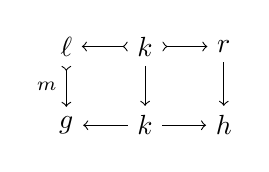
\begin{tikzpicture}
    \node (1t) at (0,1) {$ \ell $};
    \node (2t) at (1,1) {$ k $};
    \node (3t) at (2,1) {$ r $};
    \node (1b) at (0,0) {$ g $};
    \node (2b) at (1,0) {$ k $};
    \node (3b) at (2,0) {$ h $};
    \draw [>->] (2t) to node [] {\scriptsize{$  $}} (1t);
    \draw [>->] (2t) to node [] {\scriptsize{$  $}} (3t);
    \draw [->] (2b) to node [] {\scriptsize{$  $}} (1b);
    \draw [->] (2b) to node [] {\scriptsize{$  $}} (3b);
    \draw [>->] (1t) to node [left] {\scriptsize{$ m $}} (1b);
    \draw [->] (2t) to node [] {\scriptsize{$  $}} (2b);
    \draw [->] (3t) to node [] {\scriptsize{$  $}} (3b);
  \end{tikzpicture}
\]
% 
The operational viewpoint dominated in the theory of graph rewriting.
Then Gadducci and Heckel introduced an inductive viewpoint
\cite{Gadd_IndGraphTrans}. They formalize ``ranked graphs'' as arrows
in a category where the ordinary graphs are the endomorphisms on the
initial object. A ranked graph is essentially a graph with a
3-coloring on its nodes. The colors are `input', `output', and
`interior'. A graph with $ n $ input nodes and $ m $ output nodes is
thought of an arrow in a prop from $ n $ to $ m $. The composition of
ranked graphs is made by gluing the inputs of one graph to the
outputs of another. Then given a graph grammar, one then introduces a
number of 2-cells into this category in a specific way that draws a
correspondence between the rewrite relation and the arrows of the
hom-category $ \hom (0,0) $.

The next stage in the theory of rewriting is marked by the
introduction by Lack and Soboci\'{n}ski \cite{LackSobo_Adhesive} of
``adhesive categories''.  These give the most elegant axiomatization
of graph rewriting to date.  Currently, there is only a operation
perspective on adhesive rewriting.  The aim of this paper is to build
on the ideas of Gadducci and Heckel to give an inductive viewpoint on
a fragment of the theory of adhesive rewriting.

This project fits into a larger program to codify network theory into
the language of category theory
\cite{OpenPetri,RxNets,PassiveNets,NetMods,MrkvProc}.  While graphs
and similar objects play an important role in classical network
theory, we hope to move beyond such combinatorial descriptions to
understand what networks essentially are. While practitioners in many
fields use these graph-like objects to various ends, by abstracting
away the idiosyncrasies of each instance, we can study the objects
themselves.

A guiding philosophy in this program is the use of \emph{functorial
  semantics}. That is, we construct a syntax whereby systems are
arrows in a category, thus allowing for their composition which
creates larger systems.  The semantics of such systems is captured by
a functor on our syntax category from which we study properties of the
system preserved by composition; the so-called \emph{compositional
  properties}. Compositionality is desirable in the study of complex
systems because global behaviors are determined by local (read
``easier to understand'') behaviors. One source of syntax categories
is Fong's ``decorate cospans'' \cite{DecorCsp}. Another source, the
one introduced here and by Baez and Courser \cite{StrCsp} are the
\emph{structured cospan categories}.

A structured cospan builds from a pushout preserving functor
$ L \from \A \to \X $ between categories with pushouts.  The idea is
that the category $ \X $ contains the system types, the category
$ \A $ contains the interface types, and the functor $ L $ turns the
interface types into system types. A structured cospan is just a
cospan $ La \to x \gets Lb $ in the category $ \X $.  The feet of the
cospan can be thought of as identifying subsystems $ La $ and $ Lb $
of $ x $ to serve as the input and output. The compositional nature of
structured cospans can be seen if given another structured cospan
$ Lb \to y \gets Lc $ whose input matched the output of the other.
These compose as cospans typically do, giving
$ La \to x+_{Lb} y \gets Lc $.

In light of the well-developed theory or rewriting that exist for the
various graphs so prevalent in network theory, we intend to bring
rewriting into our structured cospan framework.  This brings us to the
theory of adhesive categories which requires stronger hypotheses
than those given in the above definition of a structured
cospan. Specifically, begin with a geometric morphism, that is an
adjunction $ ( L \from \A \to \X ) \dashv ( R \from \X \to \A ) $
between elementary topoi such that $ L $ preserves finite limits. In
the systems analogy, $ L $, $ \X $, and $ \A $ play the same role as
before and the compositional structure is still there.  However, we
also pursue the perspective of structured cospans as objects between
which arrows exist as commuting diagrams
%
\begin{equation} \label{eq:StrCsp-arrows}
  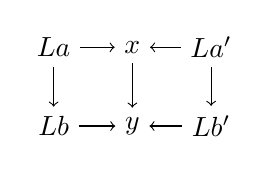
\begin{tikzpicture}
    \node (1t) at (0,1) {$ La $};
    \node (2t) at (1,1) {$ x $};
    \node (3t) at (2,1) {$ La' $};
    \node (1b) at (0,0) {$ Lb $};
    \node (2b) at (1,0) {$ y $};
    \node (3b) at (2,0) {$ Lb' $};
    \draw [->] (1t) to node [] {\scriptsize{$  $}} (2t);
    \draw [->] (3t) to node [] {\scriptsize{$  $}} (2t);
    \draw [->] (1b) to node [] {\scriptsize{$  $}} (2b);
    \draw [->] (3b) to node [] {\scriptsize{$  $}} (2b);
    \draw [->] (1t) to node [] {\scriptsize{$  $}} (1b);
    \draw [->] (2t) to node [] {\scriptsize{$  $}} (2b);
    \draw [->] (3t) to node [] {\scriptsize{$  $}} (3b);
  \end{tikzpicture}
\end{equation}
%
giving a category we denote as $ \StrCsp_L $.  Requiring that $ L $ be
a finitely continuous left adjoint ensures that $ \StrCsp_L $ is a
topos, hence adhesive \cite{LackSobo_ToposIsAdh}. This means that we
can introduce the theory of rewriting to structured cospans.

As mentioned above, the operational perspective pervades adhesive
rewriting. However, this perspective does not parallel the
compositionality present in the structured cospan formalism. The
inductive viewpoint, on the other hand, fits much more nicely into the
program of network theory as functorial semantics. Both structural
induction and compositionality involve building systems from
pieces. This is the motivation for our main result: lifting the
inductive viewpoint of graph rewriting into the context of structured
cospans.

The structure of the paper is as follows.  Section \ref{sec:StrCsp}
defines structured cospans, the main object of study. There are two
perspectives on structured cospans and we realize this by building two
separate categories.  The first category $ \StrCsp_L $, mentioned
above, has structured cospans as objects and commuting diagrams
\eqref{eq:StrCsp-arrows} as arrows. The first result, and the keystone
of the paper, is that $ \StrCsp_L $ is a topos.  This grants us access
to the theory of adhesive rewriting.  The second category, and the one
introduced by Baez and Courser \cite{StrCsp} views structured cospans
as arrows.  We then combine these two perspectives into a double
category.

In Section \ref{sec:inductive-rewriting-structured-cospans}, we sweep
over the basics of graph rewriting and cover the inductive viewpoint.
We also recall the theory of adhesive categories before applying it to
structured cospans in a categorical framework. We start with
\emph{grammars}. There are two types of grammars we are interested in.
The first involves pairing an adhesive category $ \C $ with a set of
productions $ P $ inside $ \C $. These form a category.  There is a
subcategory we use too, consisting of grammars $ ( \StrCsp_L , P ) $
where $ P $ is a set of spans in $ \StrCsp_L $ of the form
%
\[
  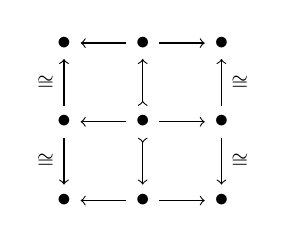
\begin{tikzpicture}
    \node (1t) at (0,2) {$ \bullet $};
    \node (2t) at (1,2) {$ \bullet $};
    \node (3t) at (2,2) {$ \bullet $};
    \node (1m) at (0,1) {$ \bullet $};
    \node (2m) at (1,1) {$ \bullet $};
    \node (3m) at (2,1) {$ \bullet $};
    \node (1b) at (0,0) {$ \bullet $};
    \node (2b) at (1,0) {$ \bullet $};
    \node (3b) at (2,0) {$ \bullet $};
    \draw [->] (2t) to node [] {\scriptsize{$  $}} (1t);
    \draw [->] (2t) to node [] {\scriptsize{$  $}} (3t);
    \draw [->] (2m) to node [] {\scriptsize{$  $}} (1m);
    \draw [->] (2m) to node [] {\scriptsize{$  $}} (3m);
    \draw [->] (2b) to node [] {\scriptsize{$  $}} (1b);
    \draw [->] (2b) to node [] {\scriptsize{$  $}} (3b);
    \draw [->] (1m) to node [left] {\scriptsize{$ \iso $}} (1t);
    \draw [->] (1m) to node [left] {\scriptsize{$ \iso $}} (1b);
    \draw [>->] (2m) to node [] {\scriptsize{$  $}} (2t);
    \draw [>->] (2m) to node [] {\scriptsize{$  $}} (2b);
    \draw [->] (3m) to node [right] {\scriptsize{$ \iso $}} (3t);
    \draw [->] (3m) to node [right] {\scriptsize{$ \iso $}} (3b);
  \end{tikzpicture}
\]
% 
and fitting them into a category $ \StrCspGram $.  Given a grammar
$ ( \C , P ) $, we define the rewriting relation on the objects
of $ \C $ using double pushouts in a manner similar to that as
was done for graphs.  However, we provide a functorial characterization
as well. Namely, the functor $ D \from \Gram \to \Gram $
that send a grammar $ ( \C , P ) $ to the grammar $ ( \C
, P') $ where a production $ g \gets d \to h $ belongs to $ P' $ if
there is a double pushout diagram
%
\[
  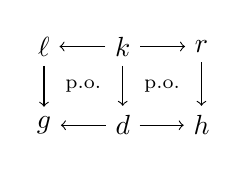
\begin{tikzpicture}
    \node (1t) at (0,1) {$ \ell $};
    \node (2t) at (1,1) {$ k $};
    \node (3t) at (2,1) {$ r $};
    \node (1b) at (0,0) {$ g $};
    \node (2b) at (1,0) {$ d $};
    \node (3b) at (2,0) {$ h $};
    \draw [->] (2t) to node [] {\scriptsize{$  $}} (1t);
    \draw [->] (2t) to node [] {\scriptsize{$  $}} (3t);
    \draw [->] (2b) to node [] {\scriptsize{$  $}} (1b);
    \draw [->] (2b) to node [] {\scriptsize{$  $}} (3b);
    \draw [->] (1t) to node [] {\scriptsize{$  $}} (1b);
    \draw [->] (2t) to node [] {\scriptsize{$  $}} (2b);
    \draw [->] (3t) to node [] {\scriptsize{$  $}} (3b);
    \node () at (0.5,0.5) {\scriptsize{p.o.}};
    \node () at (1.5,0.5) {\scriptsize{p.o.}};
  \end{tikzpicture}
\]
% 
such that the top row is a production in $ P $. We then define a
semantics functor $ S \from \Gram \to \DblCat $ valued in double
categories.  These semantics capture the compositionality of the
structured cospans and also the rewriting.  The \emph{language} of a
grammar is its image under the composite functor $ SD $. Our main
result is Theorem \ref{thm:inductive-rewriting}. Given a grammar
$ ( \X , P ) $ on a topos $ \X $ fitting into a suitable geometric
morphism $ L \dashv R \from \X \to \A $, then we construct a grammar $
( \StrCsp_L , Q ) $ such that $ g $ is related to $ h $ from the
rewriting relation on the grammar $ ( \X , P ) $ exactly when there is
a square in the double category $ SD ( \StrCsp_L , Q ) $ of the form
\[
    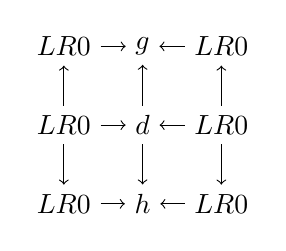
\begin{tikzpicture}
      \node (1t) at (0,2) {$ LR 0 $};
      \node (2t) at (1,2) {$ g $};
      \node (3t) at (2,2) {$ LR 0 $};
      \node (1m) at (0,1) {$ LR 0 $};
      \node (2m) at (1,1) {$ d $};
      \node (3m) at (2,1) {$ LR 0 $};
      \node (1b) at (0,0) {$ LR 0 $};
      \node (2b) at (1,0) {$ h $};
      \node (3b) at (2,0) {$ LR 0 $};
      \draw [->] (1t) to node [] {\scriptsize{$  $}} (2t);
      \draw [->] (3t) to node [] {\scriptsize{$  $}} (2t);
      \draw [->] (1m) to node [] {\scriptsize{$  $}} (2m);
      \draw [->] (3m) to node [] {\scriptsize{$  $}} (2m);
      \draw [->] (1b) to node [] {\scriptsize{$  $}} (2b);
      \draw [->] (3b) to node [] {\scriptsize{$  $}} (2b);
      \draw [->] (1m) to node [] {\scriptsize{$  $}} (1t);
      \draw [->] (1m) to node [] {\scriptsize{$  $}} (1b);
      \draw [->] (2m) to node [] {\scriptsize{$  $}} (2t);
      \draw [->] (2m) to node [] {\scriptsize{$  $}} (2b);
      \draw [->] (3m) to node [] {\scriptsize{$  $}} (3t);
      \draw [->] (3m) to node [] {\scriptsize{$  $}} (3b);
    \end{tikzpicture}
\]
Simply stated, if $ \X $ contains a type of network, then the
rewritings on networks of type $ \X $ can be understood by rewriting
on pieces of the network inside of $ ( \StrCsp , Q ) $ then gluing
them back together.

The author would like to thank John Baez and Fabio Gadducci for
helpful conversations.

% ~~~~~~~~~~~~~~~~~~~~~~~~~~~~~~~~~~~~~~~~
% ~~~~~~~~~~~ structured cospans~~~~~~~~~~
% ~~~~~~~~~~~~~~~~~~~~~~~~~~~~~~~~~~~~~~~~

\section{Structured Cospans}
\label{sec:StrCsp}

Structured cospans are introduced here, as well as by Baez and Courser
\cite{StrCsp}. Their purpose is to provide syntax for compositional
systems. Baez and Courser's work has two aims: maximize the generality
of the structured cospan construction using double categories and also
to compare structured cospans to Fong's decorated cospans
\cite{DecorCsp}. Our interests here are instead to discuss introducing
rewriting structured cospans. This requires us to make restrictions
not needed by Baez and Courser.  These restriction are harmless,
however, as most cases of interest fall within our parameters.

In this section, we make explicit two perspectives on structured
cospans.  The first is looking at structured cospans as objects of a
category with appropriate morphisms between them. The second
perspective takes structured cospans to be morphisms between
``interfaces''.  The latter perspective encode the compositional
structure.

For this section, fix an arbitrary geometric morphism
$ L \dashv R \from \X \to \A $. This is an adjunction
%
\[
  \adjunction{\X}{L}{R}{\A}
\]
%
between (elementary) topoi with $ L $ left exact. Because spans and
cospans factor heavily into this work, we use the notation
%
\(
 (f,g) \from \spn{x}{y}{z}
\)
% 
for a span
%
\[
  x \xgets{f} y \xto{g} z
\]
%
and
%
\(
  (f,g) \from \csp{x}{y}{z}
\)
% 
for a cospan
%
\[
  x \xto{f} y \xgets{g} z.
\]
% 
Because all of the categories in this paper have products and
coproducts, this notation is sensible.

% ~~~~~~~~~~~~~~~~~~~~~~~~
% ~~~~~~~~~~~~~~~~~~~~~~~~

\subsection{Structured cospans as objects}
\label{sec:StrCspAsObject}

\begin{definition}\label{df:strcsp}
  A \defn{ structured cospan } is a cospan of the form
  $ La \to x \gets Lb $. 
\end{definition}

There is no novelty in a simple cospan, but we use this language to
contextualize our work. Also, the purpose behind the restriction to a
geometric morphism is not currently clear. Let us say that this
requirement arises from practical and aesthetic considerations. For
one, a nicer theory develops, but also it is a sufficiently strong
condition to introduce rewriting of structured cospans.

Given that we are motivated by open systems, beginning by fixing
geometric morphism may signal the abstract nature of this work and
cloud the connection between structured cospans and open
systems. So that we do not drift too far from our concrete
motivations, we will draw analogies between our construction and open
systems throughout.

Here is the first such analogy. One should view the topos $ \X $ as
consisting of closed systems and their morphisms. By a \emph{closed
  system}, we mean a system that cannot interact with the outside
world. The topos $ \A $ should be thought to contain possible
interfaces for the closed systems. Equipping a closed system with an
interface provides the system a way to interact with compatible
elements of the outside world. Such a system is no longer closed, and
so we call it an \emph{open system}. The left adjoint $ L $ sends
these interfaces into $ \X $ so that they might interact with the
closed systems. The right adjoint $ R $ can be though of as returning
a closed system's largest possible interface. A word of caution: this
is an informal analogy and should only be used to gain an intuition
for the nature of structured cospans. Now, let us turn to the first of
two perspectives on structured cospans.

Through this perspective, a structured cospan consists of a closed
system $ x $ with an interface identified by the arrows from $ La $
and $ Lb $. By ignoring questions of causality, we may safely consider
$ La $ as the input to $ x $ and $ Lb $ as the output. Our open system
consists of the closed system $ x $ equipped with interface
$ La + Lb $. As expected, a morphism of open system
ought to respect these components.

\begin{definition} \label{df:morph-of-strcsp}

  A morphism from one structured cospan
  %
  \(
    \csp{La}{x}{Lb}
  \)
  %
  to another
  %
  \(
    \csp{Lc}{y}{Ld}
  \)
  % 
  is a triple of arrows $ ( f,g,h ) $ that fit into the commuting
  diagram
  \[
    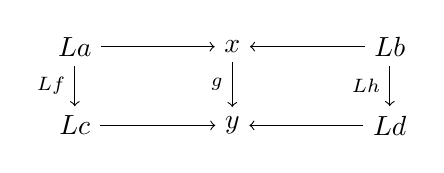
\begin{tikzpicture}
      \node (1) at (-2,1) {\( La \)};
      \node (2) at (0,1) {\( x \)};
      \node (3) at (2,1) {\( Lb \)};
      \node (4) at (-2,0) {\( Lc \)};
      \node (5) at (0,0) {\( y \)};
      \node (6) at (2,0) {\( Ld \)};
      \draw [->] (1) to node [above] {\scriptsize{\(  \)}} (2);
      \draw [->] (3) to node [above] {\scriptsize{\(  \)}} (2);
      \draw [->] (4) to node [below] {\scriptsize{\(  \)}} (5);
      \draw [->] (6) to node [below] {\scriptsize{\(  \)}} (5);
      \draw [->] (1) to node [left] {\scriptsize{\( Lf \)}} (4);
      \draw [->] (2) to node [left] {\scriptsize{\( g \)}} (5);
      \draw [->] (3) to node [left] {\scriptsize{\( Lh \)}} (6);
    \end{tikzpicture}
  \]
\end{definition}

It is a simple exercise to show that structured cospans and their
morphisms form a category.  Denote this category by $ \StrCsp_L
$. 

\begin{example}[Open graphs] \label{ex:open-graphs}

  Systems theory is intimately tied with graph theory.  A natural
  example of a structured cospan is an \emph{open graph}. While this
  notion is not new \cite{DixKiss_OpenGraphs,Gadd_IndGraphTrans}, our
  infrastructure generalizes it.

  Let
  %
  \[
    \RGraph \coloneqq [ \rgraph{\bullet}{\bullet} , \Set ]
  \]
  % 
  be the category of (directed reflexive multi-)graphs. There is an
  adjunction
  %
  \[
    \adjunction{\RGraph}{L}{R}{\Set}
  \]
  % 
  where $ Rx $ is the node set of graph $ x $ and $ La $ is the
  edgeless graph with node set $ a $. An \defn{open graph} is a cospan
  %
  \(
      \csp{La}{x}{Lb}
  \)
  % 
  for sets $ a $, $ b $, and graph $ x $. An illustrated example, with
  the reflexive loops suppressed, is
  %
  \[
    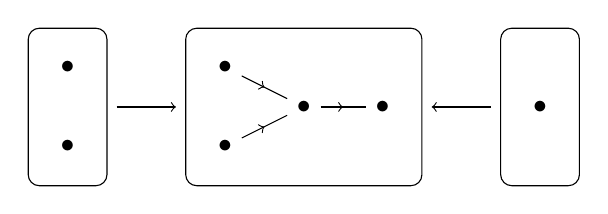
\begin{tikzpicture}
      %
      \begin{scope} % left graph
      \node (1) at (0,1) { \( \bullet \) };
      \node (2) at (0,0) { \( \bullet \) };
      \draw [rounded corners] (-0.5,-0.5) rectangle (0.5,1.5);
      \end{scope}
      %
      \begin{scope}[shift={(2,0)}] % center graph
      \node (1) at (0,1) {\( \bullet \)};
      \node (2) at (0,0) {\( \bullet \)};
      \node (3) at (1,0.5) {\( \bullet  \)};
      \node (4) at (2,0.5) {\( \bullet  \)};
      \draw [->-] (1) to (3);
      \draw [->-] (2) to (3);
      \draw [->-] (3) to (4);
      \draw [rounded corners] (-0.5,-0.5) rectangle (2.5,1.5);
      \end{scope}
      %
      \begin{scope}[shift={(6,0)}] % right graph
      \node (1) at (0,0.5) {\( \bullet \)};
      \draw [rounded corners] (-0.5,-0.5) rectangle (0.5,1.5);
      \end{scope}
      %
      \begin{scope} % graph morphisms
        \node (1) at (0.5,0.5) {};
        \node (2) at (1.5,0.5) {};
        \node (3) at (4.5,0.5) {};
        \node (4) at (5.5,0.5) {};
        \draw [->] (1) to (2);
        \draw [->] (4) to (3);
      \end{scope}
    \end{tikzpicture}
  \]
  % 
  The boxed items are graphs and the arrows between boxes are graph
  morphisms defined as suggested by the illustration.  In total, the
  three graphs and two graph morphisms make up a single open graph.
    
\end{example}

% what good is the open bit?

Having seen this example, it becomes more apparent about how open
systems can ``connect'' together. Given another open graph whose
inputs coincide with the outputs of the graph above, we can connect
the inputs and outputs together to create a new open graph. By passing
from graphs to open graphs, we are introducing
\emph{compositionality}. The category $ \StrCsp_{L} $ does not encode
the compositional structure, but we introduce a new category
$ \Csp_L $ in Section \ref{sec:strcsp-as-arrows}. Now, we show that
$ \StrCsp_L $ is a topos in a functorial way.  While interesting in
itself, this fact allows us to introduce rewriting systems to
structured cospans.

\begin{theorem}
\label{thm:strcsp-istopos}
  The category $ \StrCsp_L $ is a topos.
\end{theorem}

\begin{proof}
  The category $ \StrCsp_L $ constructed using the adjunction
  $ L \dashv R \from \X \to \A $ is equivalent to the category
  whose objects are cospans of form
  %
  \(
    \csp{a}{Rx}{b}
  \)
  % 
  and morphisms are triples $ ( f,g,h ) $ fitting into the commuting
  diagram
  %
  \[
    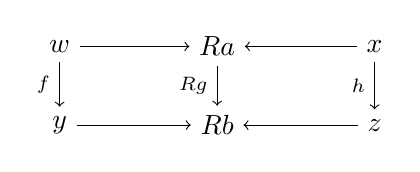
\begin{tikzpicture}
      \node (1) at (-2,1) {\( w \)};
      \node (2) at (0,1) {\( Ra \)};
      \node (3) at (2,1) {\( x \)};
      \node (4) at (-2,0) {\( y \)};
      \node (5) at (0,0) {\( Rb \)};
      \node (6) at (2,0) {\( z \)};
      \draw [->] (1) to  node [] {\scriptsize{\(  \)}} (2);
      \draw [->] (3) to node [] {\scriptsize{\(  \)}} (2);
      \draw [->] (4) to node [] {\scriptsize{\(  \)}} (5);
      \draw [->] (6) to node [] {\scriptsize{\(  \)}} (5);
      \draw [->] (1) to node [left] {\scriptsize{\( f \)}} (4);
      \draw [->] (2) to node [left] {\scriptsize{\( Rg \)}} (5);
      \draw [->] (3) to node [left] {\scriptsize{\( h \)}} (6); 
    \end{tikzpicture}
  \]
  % 
  This, in turn, is equivalent to the comma category
  $ ( \A \times \A \downarrow \Delta R ) $, where
  $ \Delta \from \A \to \A \times \A $ is the diagonal functor. But
  the diagonal functor is right adjoint to taking binary
  coproducts. That means $ \Delta R $ is also a right adjoint and,
  furthermore, that $ ( \A \times \A \downarrow \Delta R ) $ is an
  instance of Artin gluing \cite{Wraith_ArtinGlue}, hence a topos.
\end{proof}

Better yet, the construction $ \StrCsp_{(-)} $ is actually
functorial. For the following theorem, denote by $ \Topos $ the
category of elementary topoi and geometric morphisms.

\begin{theorem} \label{thm:strcsp-isfunctorial}

  There is a functor
  %
  \[
    \StrCsp_{(-)} \from
    [ \bullet \to \bullet , \Topos ]
    \to
    \Topos
  \]
  % 
  defined by  
  \[
    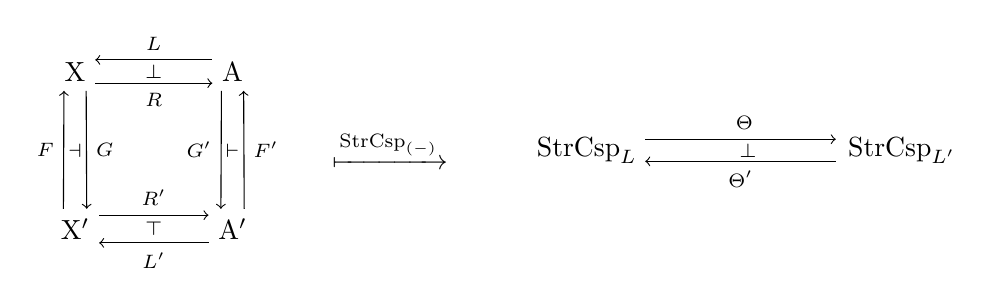
\begin{tikzpicture}
      \begin{scope}
      \node (1) at (-1,1) {\( \X \)};
      \node (2) at (-1,-1) {\( \X' \)};
      \node (3) at (1,1) {\( \A \)};
      \node (4) at (1,-1) {\( \A' \)};
      \draw [->] (1.-60) to node [right] {\scriptsize{\( G \)}} (2.60);
      \draw [<-] (1.-120) to node [left] {\scriptsize{\( F \)}} (2.120);
      \draw [<-] (1.30) to node [above] {\scriptsize{\( L \)}} (3.150);  
      \draw [->] (1.-30) to node [below] {\scriptsize{\( R \)}} (3.-150);
      \draw [->] (2.30) to node [above] {\scriptsize{\( R' \)}} (4.150);
      \draw [<-] (2.-30) to node [below] {\scriptsize{\( L' \)}} (4.-150);      
      \draw [<-] (3.-60) to node [right] {\scriptsize{\( F' \)}} (4.60);
      \draw [->] (3.-120) to node [left] {\scriptsize{\( G' \)}}
      (4.120);
      \node (5) at (0,-1) {\scriptsize{\( \top \)}};
      \node (6) at (0,1) {\scriptsize{\( \perp \)}};
      \node (7) at (-1,0) {\scriptsize{\( \dashv \)}};
      \node (8) at (1,0) {\scriptsize{\( \vdash \)}};
      \end{scope}
     % 
      \begin{scope}[shift={(3,0)}]
      \node (1) at (0,0) { $\xmapsto{ \StrCsp_{(-)} }$ };
      \end{scope}
      %
      \begin{scope}[shift={(5.5,0)}]
      \node (1) [inner sep=0.1cm] at (0,0) {\( \StrCsp_{L} \)};
      \node (2) [inner sep=0.15cm] at (4,0) {\( \StrCsp_{L'} \)};
      \node (3) at (2,0) {\scriptsize{ \( \perp \) }};
      \draw [->]
        ([yshift= 4pt]1.east) to
        node [above] {\scriptsize{ \( \Theta \) }}
        ([yshift= 4pt]2.west);
      \draw [->]
        ([yshift= -4pt]2.west) to
        node [below] {\scriptsize{ \( \Theta' \) } }
        ([yshift= -4pt]1.east);  
      \end{scope}
    \end{tikzpicture}
  \]
  % 
  which is in turn given by
  %
  \[
    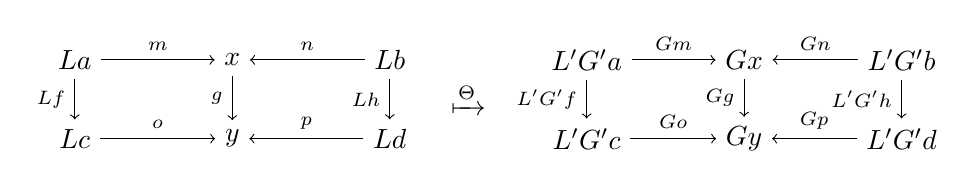
\begin{tikzpicture}
      \begin{scope}
      \node (1) at (-2,1) {\( La \)};
      \node (2) at (0,1) {\( x \)};
      \node (3) at (2,1) {\( Lb \)};
      \node (4) at (-2,0) {\( Lc \)};
      \node (5) at (0,0) {\( y \)};
      \node (6) at (2,0) {\( Ld \)};
      \draw [->] (1) to node [above] {\scriptsize{\( m \)}} (2);
      \draw [->] (3) to node [above] {\scriptsize{\( n \)}} (2);
      \draw [->] (4) to node [above] {\scriptsize{\( o \)}} (5);
      \draw [->] (6) to node [above] {\scriptsize{\( p \)}} (5);
      \draw [->] (1) to node [left] {\scriptsize{\( Lf \)}} (4);
      \draw [->] (2) to node [left] {\scriptsize{\( g \)}} (5);
      \draw [->] (3) to node [left] {\scriptsize{\( Lh \)}} (6);
      \end{scope}
      %
      \begin{scope}[shift={(3,0)}]
      \node (1) at (0,0.5) { $ \xmapsto{ \Theta } $ };
      \end{scope}
      %
      \begin{scope}[shift={(6.5,0)}]
      \node (1) at (-2,1) {\( L'G'a \)};
      \node (2) at (0,1) {\( Gx \)};
      \node (3) at (2,1) {\( L'G'b \)};
      \node (4) at (-2,0) {\( L'G'c \)};
      \node (5) at (0,0) {\( Gy \)};
      \node (6) at (2,0) {\( L'G'd \)};
      \draw [->] (1) to node [above] {\scriptsize{\( Gm \)}} (2);
      \draw [->] (3) to node [above] {\scriptsize{\( Gn \)}} (2);
      \draw [->] (4) to node [above] {\scriptsize{\( Go \)}} (5);
      \draw [->] (6) to node [above] {\scriptsize{\( Gp \)}} (5);
      \draw [->] (1) to node [left] {\scriptsize{\( L'G'f \)}} (4);
      \draw [->] (2) to node [left] {\scriptsize{\( Gg \)}} (5);
      \draw [->] (3) to node [left] {\scriptsize{\( L'G'h \)}} (6);  
      \end{scope}
    \end{tikzpicture}
  \]
  %
  and
  %
  \[
    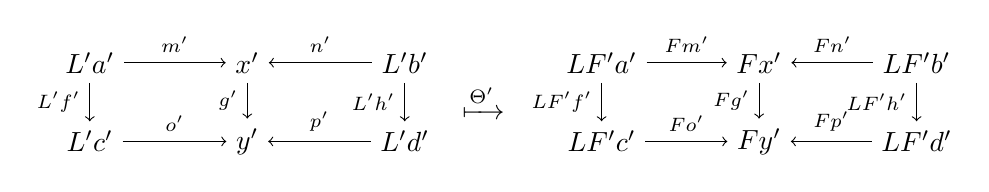
\begin{tikzpicture}
      \begin{scope}
      \node (1) at (-2,1) {\( L'a' \)};
      \node (2) at (0,1) {\( x' \)};
      \node (3) at (2,1) {\( L'b' \)};
      \node (4) at (-2,0) {\( L'c' \)};
      \node (5) at (0,0) {\( y' \)};
      \node (6) at (2,0) {\( L'd' \)};
      \draw [->] (1) to node [above] {\scriptsize{\( m' \)}} (2);
      \draw [->] (3) to node [above] {\scriptsize{\( n' \)}} (2);
      \draw [->] (4) to node [above] {\scriptsize{\( o' \)}} (5);
      \draw [->] (6) to node [above] {\scriptsize{\( p' \)}} (5);
      \draw [->] (1) to node [left] {\scriptsize{\( L'f' \)}} (4);
      \draw [->] (2) to node [left] {\scriptsize{\( g' \)}} (5);
      \draw [->] (3) to node [left] {\scriptsize{\( L'h' \)}} (6);
      \end{scope}
      %
      \begin{scope}[shift={(3,0)}]
      \node (1) at (0,0.5) { $ \xmapsto{ \Theta' } $ };
      \end{scope}
      %
      \begin{scope}[shift={(6.5,0)}]
      \node (1) at (-2,1) {\( LF'a' \)};
      \node (2) at (0,1) {\( Fx' \)};
      \node (3) at (2,1) {\( LF'b' \)};
      \node (4) at (-2,0) {\( LF'c' \)};
      \node (5) at (0,0) {\( Fy' \)};
      \node (6) at (2,0) {\( LF'd' \)};
      \draw [->] (1) to node [above] {\scriptsize{\( Fm' \)}} (2);
      \draw [->] (3) to node [above] {\scriptsize{\( Fn' \)}} (2);
      \draw [->] (4) to node [above] {\scriptsize{\( Fo' \)}} (5);
      \draw [->] (6) to node [above] {\scriptsize{\( Fp' \)}} (5);
      \draw [->] (1) to node [left] {\scriptsize{\( LF'f' \)}} (4);
      \draw [->] (2) to node [left] {\scriptsize{\( Fg' \)}} (5);
      \draw [->] (3) to node [left] {\scriptsize{\( LF'h' \)}} (6);  
      \end{scope}
    \end{tikzpicture}
  \]  
\end{theorem}

\begin{proof}
  In light of Lemma \ref{thm:strcsp-istopos}, it suffices to show that
  $ \Theta \dashv \Theta' $ gives a geometric morphism.

  Denote the structured cospans
  %
  \[
    (m,n) \colon \csp{La}{x}{Lb}
  \]
  % 
  in $ \StrCsp_{ L } $ by $ \ell $ and  
  %
  \[
    (m',n') \colon \csp{L'a'}{x'}{L'b'}
  \]
  % 
  in $ \StrCsp_{ L' } $ by $ \ell' $. Also, denote the unit and counit
  for $F \dashv G$ by $ \eta $, $ \varepsilon $ and for
  $ F' \dashv G' $ by $ \eta' $, $ \varepsilon' $.  The assignments
  %
  \begin{align}
    \left(
      ( f,g,h ) \from \ell \to \Theta' \ell'
      \right)
    & \mapsto
    \left(
      ( \varepsilon' \circ F'f , \varepsilon \circ Fg , \varepsilon'
      \circ F'h )
      \from \Theta \ell \to \ell'
      \right) \\
      %
      \left(
      ( f',g',h' ) \from \Theta \ell \to \ell'
      \right)
    & \mapsto
      \left(
      ( G'f' \circ \eta', Gg' \circ \eta , G'h' \circ \eta' )
      \from \ell \to \Theta' \ell'
      \right) 
  \end{align}
  %
  give a bijection $ \hom ( \Theta \ell , \ell' ) \simeq \hom ( \ell ,
  \Theta' \ell' ) $. Moreover, it is natural in $ \ell $ and $ \ell'
  $. This rests on the natural maps $ \eta $, $ \varepsilon $, $ \eta'
  $, and $ \varepsilon' $. The left adjoint $ \Theta' $ preserves
  finite limits because they are taken pointwise and $ L $, $ F $, and
  $ F' $ all preserve finite limits.
\end{proof}

Even though $ \StrCsp_L $ is actually a topos in our context, the
general theory of structured cospans is not beholden to toposity,
meaning that morphisms $ \StrCsp_L \to \StrCsp_{L'} $ are not
geometric morphisms. Instead, we define a \defn{structured cospan
  functor} to be a pair of finitely continuous and cocontinuous
functors $ F \from \X \to \X' $ and $ G \from \A \to \A' $ such that
$ FL=L'F $ and $ GR = R'F $.  Structured cospan categories and their
morphisms form a category, but we leave it unnamed.

% ~~~~~~~~~~~~~~~~~~~~~~~~
% ~~~~~~~~~~~~~~~~~~~~~~~~

\subsection{Structured cospans as arrows}
\label{sec:StrCsp-as-Arrows}

We now turn to capturing the compositional structure that
truly motivates the invention of structured cospans.  To do this, we
shift perspectives of structured cospans as objects in $ \StrCsp_{L} $
to structured cospans as morphisms. 

\begin{definition}
\label{def:strcsp-arr}  
  Denote by $ \Csp_{L} $ the category that has the same objects as
  $ \A $ and structured cospans $ \csp{La}{x}{Lb} $ as arrows of
  type $ a \to b $.
\end{definition}

Note that composition is defined by pushout:
%
\[
  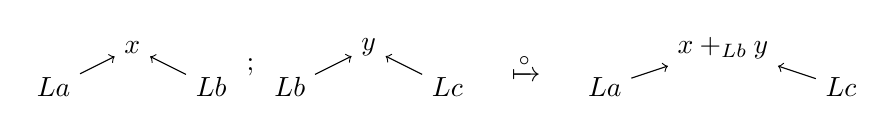
\begin{tikzpicture}
    \begin{scope}
    \node (1) at (0,0) {\( La \)};
    \node (2) at (1,0.5) {\( x \)};
    \node (3) at (2,0) {\( Lb \)};
    \node (4) at (3,0) {\( Lb \)};
    \node (5) at (4,0.5) {\( y \)};
    \node (6) at (5,0) {\( Lc \)};
    \node (7) at (2.5,0.25) {\( ; \)};
    \draw [->] (1) to node [] {\scriptsize{\(  \)}} (2);
    \draw [->] (3) to node [] {\scriptsize{\(  \)}} (2);
    \draw [->] (4) to node [] {\scriptsize{\(  \)}} (5);
    \draw [->] (6) to node [] {\scriptsize{\(  \)}} (5);
    \end{scope}
    %
    \begin{scope}[shift={(6,0)}]
    \node (1) at (0,0.25) {\( \xmapsto{\circ} \)};
    \end{scope}
    %
    \begin{scope}[shift={(7,0)}]
    \node (1) at (0,0) {\( La \)};
    \node (2) at (1.5,0.5) {\( x +_{Lb} y \)};
    \node (3) at (3,0) {\( Lc \)};
     \draw [->] (1) to node [] {\scriptsize{\(  \)}} (2);
    \draw [->] (3) to node [] {\scriptsize{\(  \)}} (2); 
    \end{scope}
  \end{tikzpicture}
\]
% 

Pushouts, in a sense, are a way of gluing things together. Hence using
pushouts as composition is a sensible way to model system
connection. Given two systems
%
\[
  \csp{La}{x}{Lb}
  \quad
  \text{ and }
  \quad
  \csp{Lb}{y}{Lc}
\]
% 
sharing a common interface $ Lb $, their composition is like
connecting at $ Lb $. To illustrate how the structured cospan
formalism allows us to connect together systems, we return to the open
graphs example.

\begin{example}
\label{ex:open-graph-as-arrow}
  The open graph
  % 
  \[
    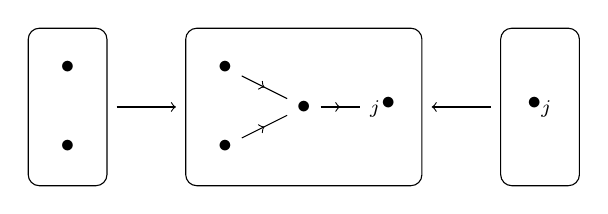
\begin{tikzpicture}
       %
      \begin{scope} % left graph
      \node (1) at (0,1) { \( \bullet \) };
      \node (2) at (0,0) { \( \bullet \) };
      \draw [rounded corners] (-0.5,-0.5) rectangle (0.5,1.5);
      \end{scope}
      %
      \begin{scope}[shift={(2,0)}] % center graph
      \node (1) at (0,1) {\( \bullet \)};
      \node (2) at (0,0) {\( \bullet \)};
      \node (3) at (1,0.5) {\( \bullet  \)};
      \node (4) at (2,0.5) {\( {}_{j} \bullet  \)};
      \draw [->-] (1) to (3);
      \draw [->-] (2) to (3);
      \draw [->-] (3) to (4);
      \draw [rounded corners] (-0.5,-0.5) rectangle (2.5,1.5);
      \end{scope}
      %
      \begin{scope}[shift={(6,0)}] % right graph
      \node (1) at (0,0.5) {\( \bullet_{j} \)};
      \draw [rounded corners] (-0.5,-0.5) rectangle (0.5,1.5);
      \end{scope}
      %
      \begin{scope} % graph morphisms
      \node (1) at (0.5,0.5) {};
      \node (2) at (1.5,0.5) {};
      \node (3) at (4.5,0.5) {};
      \node (4) at (5.5,0.5) {};
      \draw [->] (1) to (2);
      \draw [->] (4) to (3);
      \end{scope}
      %
    \end{tikzpicture}
  \]
  % 
  can be composed with the open graph
   %
  \[
    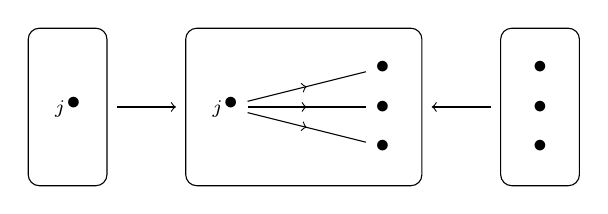
\begin{tikzpicture}
       %
      \begin{scope} % left graph
      \node (1) at (0,0.5) { \( {}_{j} \bullet \) };
      \draw [rounded corners] (-0.5,-0.5) rectangle (0.5,1.5);
      \end{scope}
      %
      \begin{scope}[shift={(2,0)}] % center graph
      \node (1) at (0,0.5) {\( {}_{j} \bullet \)};
      \node (2) at (2,0) {\( \bullet \)};
      \node (3) at (2,0.5) {\( \bullet  \)};
      \node (4) at (2,1) {\( \bullet  \)};
      \draw [->-] (1) to (2);
      \draw [->-] (1) to (3);
      \draw [->-] (1) to (4);
      \draw [rounded corners] (-0.5,-0.5) rectangle (2.5,1.5);
      \end{scope}
      %
      \begin{scope}[shift={(6,0)}] % right graph
      \node (2) at (0,0) {\( \bullet \)};
      \node (3) at (0,0.5) {\( \bullet  \)};
      \node (4) at (0,1) {\( \bullet  \)};
      \draw [rounded corners] (-0.5,-0.5) rectangle (0.5,1.5);
      \end{scope}
      %
      \begin{scope} % graph morphisms
      \node (1) at (0.5,0.5) {};
      \node (2) at (1.5,0.5) {};
      \node (3) at (4.5,0.5) {};
      \node (4) at (5.5,0.5) {};
      \draw [->] (1) to (2);
      \draw [->] (4) to (3);
      \end{scope}
      %
    \end{tikzpicture}
  \]
  %
  to obtain
  %
  \[
    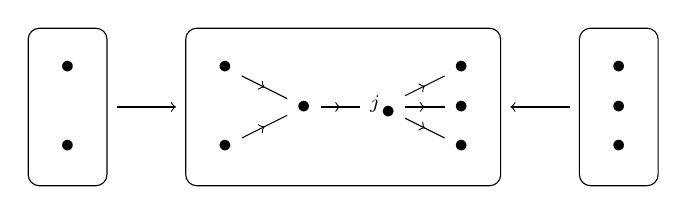
\begin{tikzpicture}
       %
      \begin{scope} % left graph
      \node (1) at (0,1) { \( \bullet \) };
      \node (2) at (0,0) { \( \bullet \) };
      \draw [rounded corners] (-0.5,-0.5) rectangle (0.5,1.5);
      \end{scope}
      %
      \begin{scope}[shift={(2,0)}] % center graph
      \node (1) at (0,1) {\( \bullet \)};
      \node (2) at (0,0) {\( \bullet \)};
      \node (3) at (1,0.5) {\( \bullet  \)};
      \node (4) at (2,0.5) {\( {}^{j} \bullet  \)};
      \node (5) at (3,0) {\( \bullet \)};
      \node (6) at (3,0.5) {\( \bullet  \)};
      \node (7) at (3,1) {\( \bullet  \)};
      \draw [->-] (1) to (3);
      \draw [->-] (2) to (3);
      \draw [->-] (3) to (4);
      \draw [->-] (4) to (5);
      \draw [->-] (4) to (6);
      \draw [->-] (4) to (7);
      \draw [rounded corners] (-0.5,-0.5) rectangle (3.5,1.5);
      \end{scope}
      %
      \begin{scope}[shift={(7,0)}] % right graph
      \node (2) at (0,0) {\( \bullet \)};
      \node (3) at (0,0.5) {\( \bullet  \)};
      \node (4) at (0,1) {\( \bullet  \)};
      \draw [rounded corners] (-0.5,-0.5) rectangle (0.5,1.5);
      \end{scope}
      %
      \begin{scope} % graph morphisms
      \node (1) at (0.5,0.5) {};
      \node (2) at (1.5,0.5) {};
      \node (3) at (5.5,0.5) {};
      \node (4) at (6.5,0.5) {};
      \draw [->] (1) to (2);
      \draw [->] (4) to (3);
      \end{scope}
      %
    \end{tikzpicture}
  \]
  %
  This composition glued the two open graphs together along the node $
  j $.
  
\end{example}

% ~~~~~~~~~~~~~~~~~~~~~~~~
% ~~~~~~~~~~~~~~~~~~~~~~~~

\subsection{A double category of structured cospans}
\label{sec:DblCatOfStrCsp}

Using double categories allows us to combine into a single instrument
the competing perspectives of structured cospans as objects and as
morphisms. For a precise definition of a symmetric monoidal double
category, we point to Shulman \cite{ShulDblCat}, though for the sake
of completeness, we list the key pieces. A double category $ \CCC $
consists of a pair of categories $ ( \C_0 , \C_1 ) $ with some
additional data that binds them together. The categories $ \C_0 $ and
$ \C_1 $ are assemble together into a double category as follows:
%
\begin{itemize}
\item the $ \CCC $-objects are exactly $ \C_0 $-the objects,
\item the $ \CCC $-vertical arrows $ c \to d $ between $ \C
  $-objects are exactly the $ \C_0 $ arrows, 
\item the $ \CCC $-horizontal arrows $ c \horarrow d $
  between $ \CCC $-objects are the $ \C_1 $-objects together with some
  structure maps assigning the domain and codomain, and
\item the squares of $ \CCC $ are
\[
  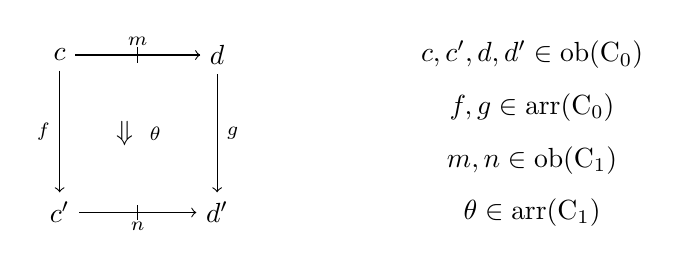
\begin{tikzpicture}
    \node (1) at (0,2) {\( c \)};
    \node (2) at (2,2) {\( d \)};
    \node (3) at (0,0) {\( c' \)};
    \node (4) at (2,0) {\( d' \)};
    \draw [-|->] (1) to node [above] {\scriptsize{\( m \)}} (2);
    \draw [->] (1) to node [left] {\scriptsize{\( f \)}} (3);
    \draw [->] (2) to node [right] {\scriptsize{\( g \)}} (4);
    \draw [-|->] (3) to node [below] {\scriptsize{\( n \)}} (4);
    \node (5) at (6,2) {\( c,c',d,d' \in \operatorname{ob} ( \C_0 ) \)};
    \node (6) at (6,1.33) {\( f,g \in \operatorname{arr} ( \C_0 ) \)};
    \node (7) at (6,.66) {\( m,n \in \operatorname{ob} ( \C_1 ) \)};
    \node (8) at (1,1) {\( \Downarrow \) \scriptsize{ \( \theta \)}};
    \node (9) at (6,0) {\( \theta \in \operatorname{arr} ( \C_1 ) \)};
  \end{tikzpicture}
\]
are the arrows of $ \C_1 $ together with structure maps attaching the
surrounding vertical arrows. 
\end{itemize}
%
The vertical arrows compose as they do in $ \C_0 $ and there is a
structure map for composing horizontal arrows. The squares can compose
both horizontally and vertically.

Observe that the horizontal arrows play two roles: as objects in their
origin category and arrows in the double category. This reflects the
content of the categories $ \StrCsp_{L} $ and $ \Csp_{L} $.

The first double category that we define is discussed in the related
work by Baez and Courser \cite[Cor.~3.9]{StrCsp}.  There, they prove
that it actually is a double category, so we content ourselves to
simply provide the definition.

\begin{definition}
  There is a double category
  $ \SSStrCsp \coloneqq ( \A , \StrCsp_{L} ) $ :
  \begin{itemize}
  \item the objects are all $ \A $-objects
  \item the vertical arrows $ a \to b $ all $ \A $-arrows, 
  \item the horizontal arrows $ \horarrow{a}{b} $ are cospans
    $ \csp{La}{x}{Lb} $, and
  \item the squares are commuting diagrams
    %
    \[
    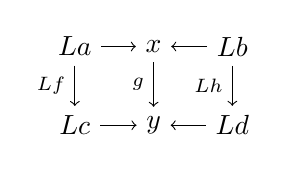
\begin{tikzpicture}
    \node (1) at (0,1) {\( La \)};
    \node (2) at (1,1) {\( x \)};
    \node (3) at (2,1) {\( Lb \)};
    \node (4) at (0,0) {\( Lc \)};
    \node (5) at (1,0) {\( y \)};
    \node (6) at (2,0) {\( Ld \)};
    \draw [->] (1) to node [] {\scriptsize{\(   \)}} (2);
    \draw [->] (3) to node [] {\scriptsize{\(  \)}} (2);
    \draw [->] (4) to node [] {\scriptsize{\(  \)}} (5);
    \draw [->] (6) to node [] {\scriptsize{\(  \)}} (5);
    \draw [->] (1) to node [left] {\scriptsize{\( Lf \)}} (4);
    \draw [->] (2) to node [left] {\scriptsize{\( g \)}} (5);
    \draw [->] (3) to node [left] {\scriptsize{\( Lh \)}} (6);
    \end{tikzpicture}
  \]
  \end{itemize}
  %  
\end{definition}

Actually, $ \SSStrCsp_L $ is a symmetric monoidal double
category. Since all involved categories are topoi, we can lift
their cocartesian structure to serve as a tensor on the double
category. However, we have no need for this structure, so we say no
more about it.

Double categories are a nice way of capturing both the object-ness and
arrow-ness of structured cospans.  An alternative would be to use
bicategories, but this doesn't reflect the nature of structured
cospans as faithfully as does double categories.

% ~~~~~~~~~~~~~~~~~~~~~~~~~~~~~~~~~~~~~~~~
% ~~~~~~~~~~~ rewriting ~~~~~~~~~~~~~~~~~~
% ~~~~~~~~~~~~~~~~~~~~~~~~~~~~~~~~~~~~~~~~

\section{Inductive Rewriting of Structured Cospans}
\label{sec:inductive-rewriting-structured-cospans}

In this final section, we recall the basics of graph rewriting and the
theorem that first provided its inductive viewpoint. We then extend
this to rewriting in a wider class of objects using the structured
cospan formalism.

\subsection{Graph rewriting}
\label{sec:Graph-Rewriting}

Graph rewriting is a well-studied field with many suitable references
\cite{Ehrig_GraphGram,DblPushoutRevis}. To be self-contained, we
present enough of the topic to facilitate a connection with our main
result.

We start our discussion of graph rewriting with the notion of a
\defn{production}: a span of graphs
%
\[
  \ell \monicgets k \monicto r
\]
%
with monic legs. Together with a \defn{matching morphism}, that is a
mono $ \ell \monicto g $, this production behaves by removing from
$ g $ the copy of $ \ell $ and replacing it with $ r $.  The removal
of $ \ell $ from $ g $ is formalized as the \defn{pushout complement}.
This is a graph $ d $ that fits into a pushout diagram
%
\[
  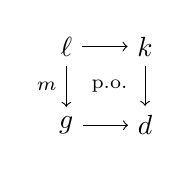
\begin{tikzpicture}
    \node (1) at (0,1) {$ \ell $};
    \node (2) at (1,1) {$ k $};
    \node (3) at (0,0) {$ g $};
    \node (4) at (1,0) {$ d $};
    \draw [->] (1) to node [] {\scriptsize{$  $}} (2);
    \draw [->] (1) to node [left] {\scriptsize{$ m $}} (3);
    \draw [->] (3) to node [] {\scriptsize{$  $}} (4);
    \draw [->] (2) to node [] {\scriptsize{$  $}} (4);
    \node () at (0.5,0.5) {\scriptsize{ p.o. }};
  \end{tikzpicture}
\]
% 
Certainly, $ d $ need not exist but when it does and
$ k \to \ell $ is monic, then $ d $ is unique up to isomorphism.

If $ P $ is a set of productions, often called a \defn{graph grammar},
there is an induced relation $ \dderiv{}{} $ on the objects of the
category $ \RGraph $. This is defined by $ \dderiv{g}{h} $ whenever
there is a production $ \spn{\ell}{k}{r} $ in $ P $, a match
$ \ell \to g $, and a pushout complement $ d $ that fit into the
double pushout diagram
%
\[
  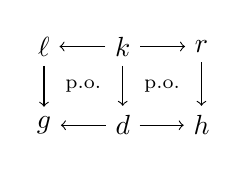
\begin{tikzpicture}
    \node (1) at (0,1) {$ \ell $};
    \node (2) at (1,1) {$ k $};
    \node (3) at (2,1) {$ r $};
    \node (4) at (0,0) {$ g $};
    \node (5) at (1,0) {$ d $};
    \node (6) at (2,0) {$ h $};
    \draw [->] (2) to node [] {\scriptsize{$  $}} (1);
    \draw [->] (2) to node [] {\scriptsize{$  $}} (3);
    \draw [->] (5) to node [] {\scriptsize{$  $}} (4);
    \draw [->] (5) to node [] {\scriptsize{$  $}} (6);
    \draw [->] (1) to node [] {\scriptsize{$  $}} (4);
    \draw [->] (2) to node [] {\scriptsize{$  $}} (5);
    \draw [->] (3) to node [] {\scriptsize{$  $}} (6);
    \node () at (0.5,0.5) {\scriptsize{p.o.}};
    \node () at (1.5,0.5) {\scriptsize{p.o.}};
  \end{tikzpicture}
\]
%
The content of this diagram is an identification of a subgraph of
shape $ \ell $ inside of $ g $, its removal and subsequent replacement
in a coherent way with $ r $, finally resulting in the graph $ h $. If
$ \dderiv{g}{h} $, we say that $ h $ is a \defn{direct derivation} of
$ g $. The term ``direct'' refers to the derivation happening in a
single step.  In general, $ \dderiv{}{} $ is not transitive, meaning
that this relation does not tell us about (multi-step) derivations. It
is also not reflexive, which is preferable for a nicer theory.
Therefore, it is customary to work with the so-called \defn{rewrite
  relation}, that is the reflexive and transitive closure
$ \deriv{}{} $. Indeed, to any graph grammar $ P $, there is an
induced rewrite relation.

In term rewriting, there are two different viewpoints. The
\emph{operational} viewpoint can be concisely described as performing
substitution. That is, we rewrite a term by substituting subterms with
other terms according to a rule. This is the viewpoint of the graph
rewriting discussed above.  On the other hand, the \emph{inductive}
viewpoint consists of building a class of rewritings from a collection
of basic ones.  This is the viewpoint that Gadducci and Heckel first
brought to graph rewriting first in \cite{Gadd_IndGraphTrans}
and we introduce to adhesive rewriting in Theorem \ref{thm:inductive-rewriting}.

To prove their result, Gadducci and Heckel made use of the following
well-known fact: the graph grammars
%
$ { k_\alpha \to \ell_\alpha \times r_\alpha } $
%
and
%
$ { ( k_\alpha )_{\flat}  \to \ell_\alpha \times r_\alpha } $,
% 
where $ ( k_\alpha )_{\flat} $ is the discrete graph underlying
$ k_\alpha $, induce the same rewrite relation
\cite[Prop.~3.3]{Ehrig_GraphGram}. Lemma
\ref{lem:production-same-rewrite-relation-as-discrete} generalizes
this result into our context.  Gadducci and Heckel leveraged this fact
to construct a computad using a graph grammar $ P $. The underlying
category of this computad is $ \Csp_L $ where $ L $ is the discrete
graph functor from Example \ref{ex:open-graphs}. We additionally add a
2-cell
%
\[
  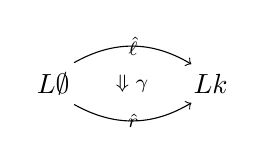
\begin{tikzpicture}
    \node (1) at (0,0) {$ L \emptyset $};
    \node (2) at (2,0) {$ Lk $};
    \node (3) at (1,0) {\scriptsize{$ \Downarrow \gamma $}};
    \draw [->, bend left] (1.45) to node [] {\scriptsize{$ \hat{\ell} $}} (2.135);
    \draw [->, bend right] (1.-45) to node [] {\scriptsize{$ \hat{r} $}} (2.-135);
  \end{tikzpicture}
\]
% 
into the computad for every production $ k \to \ell \times r $ in $ P
$. By $ \hat{\ell} $, we mean the open graph
%
\(
  \csp{L \emptyset}{\ell}{Lk}
\)
% 
and the analogous open graph for $ \hat{r} $.  Note the use of the
discrete graph underlying $ k $.  Here, we translated Gadducci and
Heckel's work into the language of structured cospans.  This computad
then freely generates a 2-category which we call $ \cat{G} $, the
1-arrows of which are open graphs. The usual closed graphs are exactly
the objects of the hom-category
$ \cat{G}( L \emptyset , L \emptyset ) $. This hom-category captures
the rewriting relation as we state here \cite[Thm.~23]{Gadd_IndGraphTran}.

\begin{theorem}
  Let $ P $ be a graph grammar. Then $ \deriv{g}{h} $ if and only
  if there is a 2-arrow from
  %
  \(
    \csp{L \emptyset}{g}{L \emptyset}
  \)
  % 
  to
  %
  \(
    \csp{L \emptyset}{h}{L \emptyset}
  \)
  % 
  in $ \cat{G} ( L \emptyset , L \emptyset ) $.  
\end{theorem}

Having shared a viewpoint on inductive graph rewriting, we now turn
to apply these ideas to inductive adhesive rewriting using structured cospans.

% ~~~~~~~~~~~~~~~~~~~~~~~~
% ~~~~~~~~~~~~~~~~~~~~~~~~

\subsection{Adhesive rewriting}
\label{sec:Adhesive-Rewriting}

There have been a number attempts at axiomatizing graph
rewriting. Adhesive categories, introduced by Lack and Soboci\'{n}ski
\cite{LackSobo_Adhesive}, is a particularly elegant solution and the
one we use presently. After recalling the basics of DPO rewriting in
adhesive categories, we use it to introduce the rewriting theory of
structured cospans.

Adhesivity is an exactness condition that ensures certain pushouts
behave as they do in $ \Set $. This is captured by saying that a
pushout satisfies the \defn{Van Kampen condition}: given a commuting cube
%
\[
  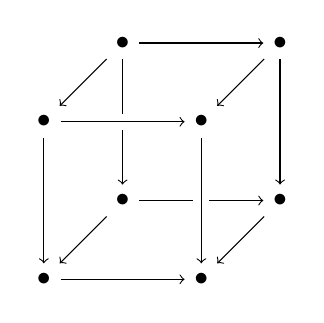
\begin{tikzpicture}
    \node (1) at (1,3) {\( \bullet \)};
    \node (2) at (0,2) {\( \bullet \)};
    \node (3) at (3,3) {\( \bullet \)};
    \node (4) at (2,2) {\( \bullet \)};
    \node (5) at (1,1) {\( \bullet \)};
    \node (6) at (0,0) {\( \bullet \)};
    \node (7) at (3,1) {\( \bullet \)};
    \node (8) at (2,0) {\( \bullet \)};
    \draw [->] (1) to node [] {\scriptsize{\(  \)}} (5);
    \draw [->] (1) to node [] {\scriptsize{\(  \)}} (2);
    \draw [->] (1) to node [] {\scriptsize{\(  \)}} (3);
    \draw [white, line width=2mm] (2) -- (4);
    \draw [->] (2) to node [] {\scriptsize{\(  \)}} (4);
    \draw [->] (3) to node [] {\scriptsize{\(  \)}} (4);
    \draw [->] (5) to node [] {\scriptsize{\(  \)}} (6);
    \draw [->] (5) to node [] {\scriptsize{\(  \)}} (7);
    \draw [->] (6) to node [] {\scriptsize{\(  \)}} (8);
    \draw [->] (7) to node [] {\scriptsize{\(  \)}} (8);
    \draw [->] (2) to node [] {\scriptsize{\(  \)}} (6);
    \draw [->] (3) to node [] {\scriptsize{\(  \)}} (7);
    \draw [white, line width=2mm] (4) -- (8);
    \draw [->] (4) to node [] {\scriptsize{\(  \)}} (8);
  \end{tikzpicture}
\]
% 
whose bottom face is the pushout and back faces are pullbacks, then
the front faces are pullbacks if and only if the top face is a pushout.

\begin{definition} \label{dfn:adhesive-category} 
  A category with pullbacks is \defn{adhesive} if pushouts along
  monics exist and are Van Kampen.
\end{definition} 

An adhesive category is a place where rewrite systems retain important
properties of DPO graph rewriting, namely concurrency. The definitions
above---production, matching morphism, pushout complement, grammar,
direct derivation, derivation, and rewrite relation---all have their
adhesive rewriting counterparts.  The primary difference is that they
occur in a generic adhesive category.

Rewriting in $ \RGraph $ had the benefit of being able to describe a
production's behavior by referring to edges and nodes. While we lose
this ability having abstracted to adhesive categories, the intuition
of removing a subobject and coherently replacing it with another
is helpful.

It is still true that pushout complements, if they exist, over a mono
are unique up to isomorphism \cite[Lem.~15]{LackSobo_Adhesive}

For improved bookkeeping, we pair a grammar with the adhesive category
housing the productions. Specifically, a production is a pair $ ( \C ,
P) $ where $ \C $ is an adhesive category and $ P $ is a set of
productions in $ \C $. This pairing allows us to define the following category.

\begin{definition}
  There is a category $ \Gram $ having
  \begin{itemize}
  \item as object grammars $ ( \C , P ) $, and
  \item as arrows $ ( \C , P ) \to ( \D , Q ) $ functors $ F \from
    \C \to D $ such that $ FP \subseteq Q $.
  \end{itemize}
\end{definition}

As in graph rewriting, any grammar $ ( \C , P ) $ induces a relation
on the objects of $ \C $ defined by $ \dderiv{g}{h} $ whenever there
is a production $ \spn{g}{d}{h} $ fitting into the bottom row of a
double pushout diagram
%
\[
  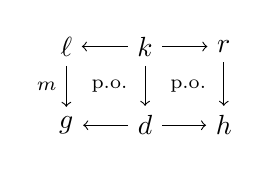
\begin{tikzpicture}
    \node (1) at (0,1) {\( \ell \)};
    \node (2) at (1,1) {\( k \)};
    \node (3) at (2,1) {\( r \)};
    \node (4) at (0,0) {\( g \)};
    \node (5) at (1,0) {\( d \)};
    \node (6) at (2,0) {\( h \)};
    \draw [->] (2) to node [] {\scriptsize{\( \)}} (1);
    \draw [->] (2) to node [] {\scriptsize{\( \)}} (3);
    \draw [->] (5) to node [] {\scriptsize{\( \)}} (4);
    \draw [->] (5) to node [] {\scriptsize{\( \)}} (6);
    \draw [->] (1) to node [left] {\scriptsize{\( m \)}} (4);
    \draw [->] (2) to node [] {\scriptsize{\( \)}} (5);
    \draw [->] (3) to node [] {\scriptsize{\( \)}} (6);
    \node () at (0.5,0.5) {\scriptsize{ p.o.\ }};
    \node () at (1.5,0.5) {\scriptsize{ p.o.\ }};
  \end{tikzpicture}
\]
% 
such that the top row is a production in $ P $ and $ m $ is monic. In
fact, this relation arises from a functor as shown in the following lemma. 

\begin{lemma}
  There is an idempotent functor $ D \from \Gram \to \Gram $, called
  the \defn{direct derivation functor}, defined on objects by setting
  $ D ( \C , P ) $ to be the grammar in $ \C $ consisting of all
  productions $ \spn{g}{h}{d} $ that witness the relation
  $ \dderiv{g}{h} $ with respect to $ ( \C , P ) $. On arrows,
  $ DF \from D( \C , P ) \to D( \D , Q ) $ is defined exactly as
  $ F $.  Moreover, the identity on $ \Gram $ is a subfunctor of
  $ D $.
\end{lemma}

\begin{proof}
  That $ D ( \C , P ) $ actually gives a grammar follows from the fact
  that pushouts respect monics in an adhesive category
  \cite[Lem.~12]{LackSobo_Adhesive}.
  
  That $ D $ is idempotent is equivalent to saying that, for a set
  $ P $ of productions, $ \dderiv{g}{h} $ with respect to
  $ D ( \C , P ) $ if and only if $ \dderiv{g}{h} $ with respect to
  $ DD ( \C , P ) $. This follows from the fact that the outer box of
  the diagram
    %
    \[
      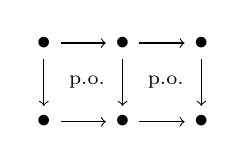
\begin{tikzpicture}
        \node (1) at (0,1) {\( \bullet \)};
        \node (2) at (1,1) {\( \bullet \)};
        \node (3) at (2,1) {\( \bullet \)};
        \node (4) at (0,0) {\( \bullet \)};
        \node (5) at (1,0) {\( \bullet \)};
        \node (6) at (2,0) {\( \bullet \)};
        \draw [->] (1) to node [] {\scriptsize{\(  \)}} (2);
        \draw [->] (2) to node [] {\scriptsize{\(  \)}} (3);
        \draw [->] (4) to node [] {\scriptsize{\(  \)}} (5);
        \draw [->] (5) to node [] {\scriptsize{\(  \)}} (6);
        \draw [->] (1) to node [] {\scriptsize{\(  \)}} (4);
        \draw [->] (2) to node [] {\scriptsize{\(  \)}} (5);
        \draw [->] (3) to node [] {\scriptsize{\(  \)}} (6);
        \node () at (0.5,0.5) {\scriptsize{ p.o.\ }};
        \node () at (1.5,0.5) {\scriptsize{ p.o.\ }};
      \end{tikzpicture}
    \]
    %
    is a pushout.

    The identity is a subfunctor of $ D $ because $ \dderiv{\ell}{r} $
    for any production $ \spn{\ell }{k}{r} $ in $ ( \C , P ) $ via a
    triple of identity arrows. Hence the identity functor on $ \C $
    turns $ ( \C , P ) $ into a subobject of $ D ( \C , P ) $.  
\end{proof}

As in the graph rewriting case, we are actually interested in the
rewriting relation $ \deriv{}{} $ defined to be the reflexive
transitive closure of $ \dderiv{}{} $.  A useful fact that we use in
our main result is that the rewriting relation plays well with
coproducts.

\begin{lemma}
\label{thm:rewrite-rel-is-additive}
  If $ \deriv{x}{y} $ and $ \deriv{x'}{y'} $, then $ \deriv{x+x'}{y+y'} $
\end{lemma}

\begin{proof}
  It the derivation $ \deriv{x}{y} $ comes from a string of double
  pushout diagrams
  %
  \[
    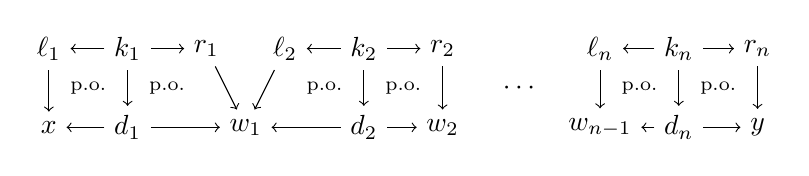
\begin{tikzpicture}
      \node (1t) at (0,1) {$ \ell_1 $};
      \node (2t) at (1,1) {$ k_1 $};
      \node (3t) at (2,1) {$ r_1 $};
      \node (4t) at (3,1) {$ \ell_2 $};
      \node (5t) at (4,1) {$ k_2 $};
      \node (6t) at (5,1) {$ r_2 $};
      \node (7t) at (7,1) {$ \ell_n $};
      \node (8t) at (8,1) {$ k_n $};
      \node (9t) at (9,1) {$ r_n $};
      \node (1b) at (0,0) {$ x $};
      \node (2b) at (1,0) {$ d_1 $};
      \node (3b) at (2.5,0) {$ w_1 $};
      \node (4b) at (4,0) {$ d_2 $};
      \node (5b) at (5,0) {$ w_2 $};
      \node (6b) at (7,0) {$ w_{n-1} $};
      \node (7b) at (8,0) {$ d_n $};
      \node (8b) at (9,0) {$ y $};
      \draw [->] (2t) to node [] {\scriptsize{$  $}} (1t);
      \draw [->] (2t) to node [] {\scriptsize{$  $}} (3t);
      \draw [->] (5t) to node [] {\scriptsize{$  $}} (4t);
      \draw [->] (5t) to node [] {\scriptsize{$  $}} (6t);
      \draw [->] (8t) to node [] {\scriptsize{$  $}} (7t);
      \draw [->] (8t) to node [] {\scriptsize{$  $}} (9t);
      \draw [->] (2b) to node [] {\scriptsize{$  $}} (1b);
      \draw [->] (2b) to node [] {\scriptsize{$  $}} (3b);
      \draw [->] (4b) to node [] {\scriptsize{$  $}} (3b);
      \draw [->] (4b) to node [] {\scriptsize{$  $}} (5b);
      \draw [->] (7b) to node [] {\scriptsize{$  $}} (6b);
      \draw [->] (7b) to node [] {\scriptsize{$  $}} (8b);
      \draw [->] (1t) to node [] {\scriptsize{$  $}} (1b);
      \draw [->] (2t) to node [] {\scriptsize{$  $}} (2b);
      \draw [->] (3t) to node [] {\scriptsize{$  $}} (3b);
      \draw [->] (4t) to node [] {\scriptsize{$  $}} (3b);
      \draw [->] (5t) to node [] {\scriptsize{$  $}} (4b);
      \draw [->] (6t) to node [] {\scriptsize{$  $}} (5b);
      \draw [->] (7t) to node [] {\scriptsize{$  $}} (6b);
      \draw [->] (8t) to node [] {\scriptsize{$  $}} (7b);
      \draw [->] (9t) to node [] {\scriptsize{$  $}} (8b);
      \node () at (6,0.5) {$ \dotsm $};
      \node () at (0.5,0.5) {\scriptsize{p.o.}};
      \node () at (1.5,0.5) {\scriptsize{p.o.}};
      \node () at (3.5,0.5) {\scriptsize{p.o.}};
      \node () at (4.5,0.5) {\scriptsize{p.o.}};
      \node () at (7.5,0.5) {\scriptsize{p.o.}};
      \node () at (8.5,0.5) {\scriptsize{p.o.}};
    \end{tikzpicture}
  \]
  %
  and the derivation $ \deriv{x}{y} $ comes from a string of double
  pushout diagrams
  %
  \[
    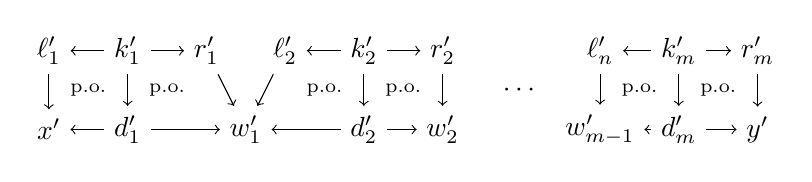
\begin{tikzpicture}
      \node (1t) at (0,1) {$ \ell'_1 $};
      \node (2t) at (1,1) {$ k'_1 $};
      \node (3t) at (2,1) {$ r'_1 $};
      \node (4t) at (3,1) {$ \ell'_2 $};
      \node (5t) at (4,1) {$ k'_2 $};
      \node (6t) at (5,1) {$ r'_2 $};
      \node (7t) at (7,1) {$ \ell'_n $};
      \node (8t) at (8,1) {$ k'_m $};
      \node (9t) at (9,1) {$ r'_m $};
      \node (1b) at (0,0) {$ x' $};
      \node (2b) at (1,0) {$ d'_1 $};
      \node (3b) at (2.5,0) {$ w'_1 $};
      \node (4b) at (4,0) {$ d'_2 $};
      \node (5b) at (5,0) {$ w'_2 $};
      \node (6b) at (7,0) {$ w'_{m-1} $};
      \node (7b) at (8,0) {$ d'_m $};
      \node (8b) at (9,0) {$ y' $};
      \draw [->] (2t) to node [] {\scriptsize{$  $}} (1t);
      \draw [->] (2t) to node [] {\scriptsize{$  $}} (3t);
      \draw [->] (5t) to node [] {\scriptsize{$  $}} (4t);
      \draw [->] (5t) to node [] {\scriptsize{$  $}} (6t);
      \draw [->] (8t) to node [] {\scriptsize{$  $}} (7t);
      \draw [->] (8t) to node [] {\scriptsize{$  $}} (9t);
      \draw [->] (2b) to node [] {\scriptsize{$  $}} (1b);
      \draw [->] (2b) to node [] {\scriptsize{$  $}} (3b);
      \draw [->] (4b) to node [] {\scriptsize{$  $}} (3b);
      \draw [->] (4b) to node [] {\scriptsize{$  $}} (5b);
      \draw [->] (7b) to node [] {\scriptsize{$  $}} (6b);
      \draw [->] (7b) to node [] {\scriptsize{$  $}} (8b);
      \draw [->] (1t) to node [] {\scriptsize{$  $}} (1b);
      \draw [->] (2t) to node [] {\scriptsize{$  $}} (2b);
      \draw [->] (3t) to node [] {\scriptsize{$  $}} (3b);
      \draw [->] (4t) to node [] {\scriptsize{$  $}} (3b);
      \draw [->] (5t) to node [] {\scriptsize{$  $}} (4b);
      \draw [->] (6t) to node [] {\scriptsize{$  $}} (5b);
      \draw [->] (7t) to node [] {\scriptsize{$  $}} (6b);
      \draw [->] (8t) to node [] {\scriptsize{$  $}} (7b);
      \draw [->] (9t) to node [] {\scriptsize{$  $}} (8b);
      \node () at (6,0.5) {$ \dotsm $};
      \node () at (0.5,0.5) {\scriptsize{p.o.}};
      \node () at (1.5,0.5) {\scriptsize{p.o.}};
      \node () at (3.5,0.5) {\scriptsize{p.o.}};
      \node () at (4.5,0.5) {\scriptsize{p.o.}};
      \node () at (7.5,0.5) {\scriptsize{p.o.}};
      \node () at (8.5,0.5) {\scriptsize{p.o.}};
    \end{tikzpicture}
  \]
  % 
  then $ \deriv{x+x'}{y+y'} $ is realized by concatenating to the end
  of first string with $ x' $ summed with the bottom row the second
  string with $ y $ summed on the bottom row.
\end{proof}

We can obtain $ \deriv{}{} $ functorially by viewing the productions
as arrows in a span category.

\begin{lemma}
  There is a functor $ S \from \Gram \to \Cat $, defined on objects by
  setting $ S ( \C , P ) $ to be the subcategory of $ \Span ( \C ) $
  generated by the productions in $ P $ and on arrows by setting
  $ SF \from S ( \C , P ) \to S ( \D , Q ) $ to be the functor
  given by $ SFc = Fc $ and
  %
  \[
    ( c \xgets{f} d \xto{g} e )
    \mapsto
    ( Fc \xgets{Ff} Fd \xto{Fg} Fe )
  \]
\end{lemma}

For expositional purposes, we will denote the composite functor $ SD $
by $ \Lang $ and call $ \Lang ( \C , P ) $ the \defn{language} of
$ ( \C , P ) $. The language is another characterization of the
rewrite relation.

\begin{theorem}
  $ \deriv{g}{h} $ with respect to a grammar $ ( \C , P ) $ if and
  only if there is an arrow $ g \to h $ in $ \Lang ( \C , P ) $.
\end{theorem}

\begin{proof}
  If $ \deriv{g}{h} $, then there is a zig-zag from $ g $ to $ h $
  comprised of productions in $ D ( \C , P ) $ and identity spans.
  This zig-zag gives a sequence of composable arrows in
  $ \Lang ( \C , P ) $.  Conversely, any arrow $ g \to h $ in
  $ \Lang ( \C , P ) $ is a composite of generating arrows.
\end{proof}

% ~~~~~~~~~~~~~~~~~~~~~~~~
% ~~~~~~~~~~~~~~~~~~~~~~~~

\subsection{Rewriting structured cospans}
\label{sec:Rewriting-StrCsp}

Having built up the necessary infrastructure, we now turn to rewriting
structured cospans. To do this we need structured cospans to form an
adhesive category. Theorem \ref{thm:strcsp-istopos} together with the
fact that topoi are adhesive \cite{LackSobo_ToposIsAdh} gives the
following result.

\begin{theorem} \label{thm:dpo_category-StrCsp-adhsv}
  The category $ \StrCsp_{L} $ is adhesive for any geometric morphism
  $ L \dashv R $.
\end{theorem}

This ensures that we are within reasonable
constraints to define rewriting on structured cospans. The language
$ \Lang ( \StrCsp_{L} , P ) $ is a subcategory of
$ \Span ( \StrCsp_{L} ) $ generated by spans of structured cospans,
that is commuting diagrams of form
%
\[
  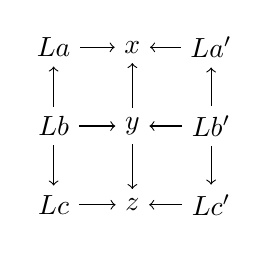
\begin{tikzpicture}
    \node (1) at (0,2) {\( La \)};
    \node (2) at (1,2) {\( x \)};
    \node (3) at (2,2) {\( La' \)};
    \node (4) at (0,1) {\( Lb \)};
    \node (5) at (1,1) {\( y \)};
    \node (6) at (2,1) {\( Lb' \)};
    \node (7) at (0,0) {\( Lc \)};
    \node (8) at (1,0) {\( z \)};
    \node (9) at (2,0) {\( Lc' \)};
    \draw [->] (1) to node [] {\scriptsize{\(  \)}} (2);
    \draw [->] (3) to node [] {\scriptsize{\(  \)}} (2);
    \draw [->] (4) to node [] {\scriptsize{\(  \)}} (5);
    \draw [->] (6) to node [] {\scriptsize{\(  \)}} (5);
    \draw [->] (7) to node [] {\scriptsize{\(  \)}} (8);
    \draw [->] (9) to node [] {\scriptsize{\(  \)}} (8);
    \draw [->] (4) to node [] {\scriptsize{\(  \)}} (1);
    \draw [->] (4) to node [] {\scriptsize{\(  \)}} (7);
    \draw [->] (5) to node [] {\scriptsize{\(  \)}} (2);
    \draw [->] (5) to node [] {\scriptsize{\(  \)}} (8);
    \draw [->] (6) to node [] {\scriptsize{\(  \)}} (3);
    \draw [->] (6) to node [] {\scriptsize{\(  \)}} (9); 
  \end{tikzpicture}
\]
% 
This is an arrow from $ \csp{La}{x}{La'}$ to $ \csp{Lc}{z}{Lc'} $. In
this span category, we can compose productions, but not structured
cospans.  To accommodate both compositions, we use the theory of
double categories.

To use double categories, we need to restrict the class of grammars
that we work with.  Fortunately, the resulting language is
structurally richer. 

\begin{definition} \label{def:linear-grammars}
  %
  The category of \defn{structured cospan grammars} $ \StrCspGram $ is
  a subcategory of $ \Gram $.  The objects are $ ( \StrCsp_{L} , P ) $
  where $ P $ consists of productions of the form
  %
  \[
    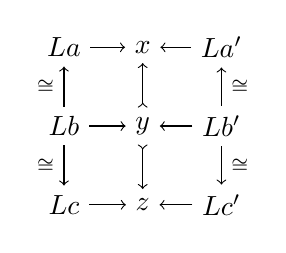
\begin{tikzpicture}
      \begin{scope}
        \node (1) at (0,2) {\( La \)};
        \node (2) at (1,2) {\( x \)};
        \node (3) at (2,2) {\( La' \)};
        \node (4) at (0,1) {\( Lb \)};
        \node (5) at (1,1) {\( y \)};
        \node (6) at (2,1) {\( Lb' \)};
        \node (7) at (0,0) {\( Lc \)};
        \node (8) at (1,0) {\( z \)};
        \node (9) at (2,0) {\( Lc' \)};
        \draw [->] (1) to node []
          {\scriptsize{\( \)}} (2);
        \draw [->] (3) to node []
          {\scriptsize{\( \)}} (2);
        \draw [->] (4) to node []
          {\scriptsize{\( \)}} (5);
        \draw [->] (6) to node []
          {\scriptsize{\( \)}} (5);
        \draw [->] (7) to node []
          {\scriptsize{\( \)}} (8);
        \draw [->] (9) to node []
          {\scriptsize{\( \)}} (8);
        \draw [->] (4) to node [left]
          {\scriptsize{\( \iso \)}} (1);
        \draw [->] (4) to node [left]
          {\scriptsize{\( \iso \)}} (7);
        \draw [>->] (5) to node []
          {\scriptsize{\( \)}} (2);
        \draw [>->] (5) to node []
          {\scriptsize{\( \)}} (8);
        \draw [->] (6) to node [right]
          {\scriptsize{\( \iso \)}} (3);
        \draw [->] (6) to node [right]
          {\scriptsize{\( \iso \)}} (9);
      \end{scope}
    \end{tikzpicture}
  \]
  %
  and the morphisms are the structured cospan functors that are stable
  under the productions.
  % 
\end{definition}

Following our work in adhesive rewriting, we define a language for the
structure cospan grammars. However, instead of a category-valued
semantics, we provide a double category semantics. Specifically, the
language functor is the composite of two functors:
$ D \from \StrCspGram \to \StrCspGram $, which is a restriction of the
associated functor defined in Section \ref{sec:Graph-Rewriting} and
the functor $ S \from \StrCspGram \to \DblCat $.

To define $ S $, we reference the double category $ \MonSpCsp (\C) $
for a topos $ \C $ introduced in \cite{CicCour_SpCspTopos}.  The
objects are from $ \C $, the vertical arrows are spans in $ \C $ with
invertible legs, the horizontal arrows are cospans in $ \C $, and the
squares are monic legged spans of cospans in $ \C $. The latter are
diagrams with shape
%
\[
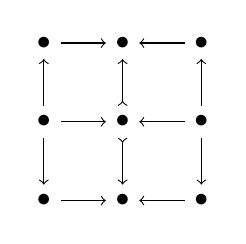
\begin{tikzpicture}
  \node (00) at (0,0) {$ \bullet $};
  \node (01) at (0,1) {$ \bullet $};
  \node (02) at (0,2) {$ \bullet $};
  \node (10) at (1,0) {$ \bullet $};
  \node (11) at (1,1) {$ \bullet $};
  \node (12) at (1,2) {$ \bullet $};
  \node (20) at (2,0) {$ \bullet $};
  \node (21) at (2,1) {$ \bullet $};
  \node (22) at (2,2) {$ \bullet $};
  \draw [->] (02) to node [] {\scriptsize{$  $}} (12);
  \draw [->] (22) to node [] {\scriptsize{$  $}} (12);
  \draw [->] (01) to node [] {\scriptsize{$  $}} (11);
  \draw [->] (21) to node [] {\scriptsize{$  $}} (11);
  \draw [->] (00) to node [] {\scriptsize{$  $}} (10);
  \draw [->] (20) to node [] {\scriptsize{$  $}} (10);
  \draw [->] (01) to node [] {\scriptsize{$  $}} (02);
  \draw [->] (01) to node [] {\scriptsize{$  $}} (00);
  \draw [>->] (11) to node [] {\scriptsize{$  $}} (12);
  \draw [>->] (11) to node [] {\scriptsize{$  $}} (10);
  \draw [->] (21) to node [] {\scriptsize{$  $}} (22);
  \draw [->] (21) to node [] {\scriptsize{$  $}} (20);
\end{tikzpicture}
\]
%

Given a structured cospan grammar $ ( \StrCsp_L , P ) $, observe that
the productions in $ P $ are admissible as squares in
$ \MonSpCsp (\X) $. Denote by $ S ( \StrCsp_L , P ) $ the sub-double
category of $ \MonSpCsp ( \X ) $ that is full on objects, vertical and
horizontal arrows, and generated by the productions in
$ P $. This assignment is functorial
%
\todo{double check this}
%
because
%
\[
  (F,G) \from ( \StrCsp_{L} , P ) \to ( \StrCsp_{L'} , P' )
\]
% 
gives a mapping between the generators of $ S ( \StrCsp_{L} , P ) $
and $ S ( \StrCsp_{L'} , P' ) $.  Composition holds because
$ F $ and $ G $ are both preserve pullbacks and pushouts. This allows
us to define the language functor $ \Lang \coloneqq SD $.  

For the following theorem, we denote by $ ( \C , P_{\flat} ) $ the
\defn{discrete adhesive grammar} underlying the adhesive grammar $ (
\C , P ) $. The discrete adhesive grammar consists of productions $
LRK \to k \to \ell \times r $ for each $ k \to \ell \times r $ in $ P $. 

For the next lemma, we recall that a poset is \textbf{well-founded} if
every non-empty subset has a minimal element.  Whenever the axiom of
choice is present, well-foundedness is equivalent to the lack of
infinite descending chains. For a relevant example, aAs the axiom of
choice holds in any presheaf, the Heyting algebra $ \Sub ( x ) $ for
any finite-set valued presheaf $ x $ is well-founded.

\begin{lemma}
\label{lem:production-same-rewrite-relation-as-discrete}
Fix a geometric morphism $ L \dashv R \from \X \to \A $ with monic
counit. Let $ ( \X , P ) $ be a grammar such that for every
$ \X $-object $ x $ in the apex of a production of $ P $, the Heyting
algebra $ \Sub (x) $ is well-founded.  The rewriting relation for an
adhesive grammar $ ( \X , P ) $ is equal to rewriting relation for the
discrete adhesive grammar $ ( \X , P_{\flat} ) $
\end{lemma}

\begin{proof}
  For any derivation
  %
  \[
  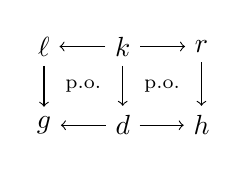
\begin{tikzpicture}
    \node (1t) at (0,1) {$ \ell $};
    \node (2t) at (1,1) {$ k $};
    \node (3t) at (2,1) {$ r $};
    \node (1b) at (0,0) {$ g $};
    \node (2b) at (1,0) {$ d $};
    \node (3b) at (2,0) {$ h $};
    \draw [->] (2t) to node [] {\scriptsize{$  $}} (1t);
    \draw [->] (2t) to node [] {\scriptsize{$  $}} (3t);
    \draw [->] (2b) to node [] {\scriptsize{$  $}} (1b);
    \draw [->] (2b) to node [] {\scriptsize{$  $}} (3b);
    \draw [->] (1t) to node [] {\scriptsize{$  $}} (1b);
    \draw [->] (2t) to node [] {\scriptsize{$  $}} (2b);
    \draw [->] (3t) to node [] {\scriptsize{$  $}} (3b);
    \node () at (0.5,0.5) {\scriptsize{p.o.}};
    \node () at (1.5,0.5) {\scriptsize{p.o.}};
  \end{tikzpicture}
  \]
  % 
  arising from $ P $, there is a derivation
  %
  \[
  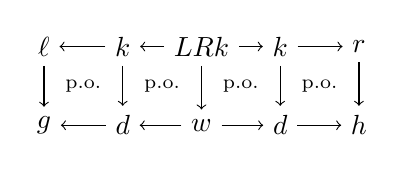
\begin{tikzpicture}
    \node (01) at (0,1) {$ \ell $};
    \node (11) at (1,1) {$ k $};
    \node (21) at (2,1) {$ LRk $};
    \node (31) at (3,1) {$ k $};
    \node (41) at (4,1) {$ r $};
    \node (00) at (0,0) {$ g $};
    \node (10) at (1,0) {$ d $};
    \node (20) at (2,0) {$ w $};
    \node (30) at (3,0) {$ d $};
    \node (40) at (4,0) {$ h $};
    \draw [->] (11) to node [] {\scriptsize{$  $}} (01);
    \draw [->] (21) to node [] {\scriptsize{$  $}} (11);
    \draw [->] (21) to node [] {\scriptsize{$  $}} (31);
    \draw [->] (31) to node [] {\scriptsize{$  $}} (41);
    \draw [->] (10) to node [] {\scriptsize{$  $}} (00);
    \draw [->] (20) to node [] {\scriptsize{$  $}} (10);
    \draw [->] (20) to node [] {\scriptsize{$  $}} (30);
    \draw [->] (30) to node [] {\scriptsize{$  $}} (40);
    \draw [->] (01) to node [] {\scriptsize{$  $}} (00);
    \draw [->] (11) to node [] {\scriptsize{$  $}} (10);
    \draw [->] (21) to node [] {\scriptsize{$  $}} (20);
    \draw [->] (31) to node [] {\scriptsize{$  $}} (30);
    \draw [->] (41) to node [] {\scriptsize{$  $}} (40);
    \node () at (0.5,0.5) {\scriptsize{p.o.}};
    \node () at (1.5,0.5) {\scriptsize{p.o.}};
    \node () at (2.5,0.5) {\scriptsize{p.o.}};
    \node () at (3.5,0.5) {\scriptsize{p.o.}};
  \end{tikzpicture}
  \]
  %
  where 
  %
  \[
    w \coloneqq
    \bigwedge \{ z \colon z \wedge k = x \} \vee LRk.
  \]
  Note that $ w \vee k = x $ and $ w \wedge k = LRy $ which gives that
  the two inner squares of the lower diagram are pushouts.
\end{proof}

Let us now connect rewriting structured cospans to rewriting in a
topos. Fix a geometric morphism $ L \dashv R \from \X \to \A $ and
grammar $ ( \X , P ) $ satisfying the conditions of Lemma
\ref{lem:production-same-rewrite-relation-as-discrete}.  Associate to
$ ( \X , P ) $ a structured cospan grammar $ ( \StrCsp_L , P' ) $
consisting of a production
%
\[
  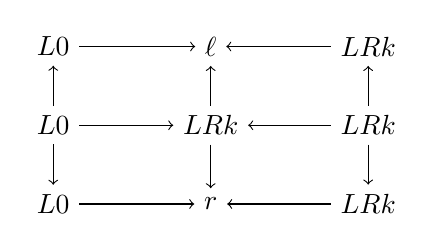
\begin{tikzpicture}
    \node (1) at (0,2) {$ L 0 $};
    \node (2) at (2,2) {$ \ell $};
    \node (3) at (4,2) {$ LRk $};
    \node (4) at (0,1) {$ L 0 $};
    \node (5) at (2,1) {$ LRk $};
    \node (6) at (4,1) {$ LRk $};
    \node (7) at (0,0) {$ L 0 $};
    \node (8) at (2,0) {$ r $};
    \node (9) at (4,0) {$ LRk $};
    \draw [->] (1) to node [] {\scriptsize{$  $}} (2);
    \draw [->] (3) to node [] {\scriptsize{$  $}} (2);
    \draw [->] (4) to node [] {\scriptsize{$  $}} (5);
    \draw [->] (6) to node [] {\scriptsize{$  $}} (5);
    \draw [->] (7) to node [] {\scriptsize{$  $}} (8);
    \draw [->] (9) to node [] {\scriptsize{$  $}} (8);
    \draw [->] (4) to node [] {\scriptsize{$  $}} (1);
    \draw [->] (4) to node [] {\scriptsize{$  $}} (7);
    \draw [->] (5) to node [] {\scriptsize{$  $}} (2);
    \draw [->] (5) to node [] {\scriptsize{$  $}} (8);
    \draw [->] (6) to node [] {\scriptsize{$  $}} (3);
    \draw [->] (6) to node [] {\scriptsize{$  $}} (9);
  \end{tikzpicture}
\]
% 
for every production $ LRk \to \ell \times r $ of $ P_{\flat} $. The
main theorem encodes the rewrite relation from $ ( \X , P ) $ in the
double category $ \Lang ( \StrCsp_L , P' ) $.

\begin{theorem} \label{thm:inductive-rewriting}
  Fix a geometric morphism $ L \dashv R \from \X \to \A $ and grammar
  $ ( \X , P ) $ satisfying the conditions of Lemma
  \ref{lem:production-same-rewrite-relation-as-discrete}. Then
  $ \deriv{g}{h} $ in the rewriting relation for an grammar
  $ ( \X , P ) $ if and only if there is a square
  %
  \[
    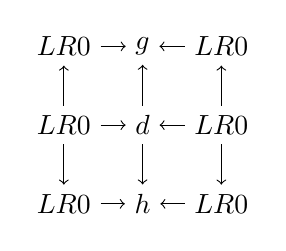
\begin{tikzpicture}
      \node (1t) at (0,2) {$ LR 0 $};
      \node (2t) at (1,2) {$ g $};
      \node (3t) at (2,2) {$ LR 0 $};
      \node (1m) at (0,1) {$ LR 0 $};
      \node (2m) at (1,1) {$ d $};
      \node (3m) at (2,1) {$ LR 0 $};
      \node (1b) at (0,0) {$ LR 0 $};
      \node (2b) at (1,0) {$ h $};
      \node (3b) at (2,0) {$ LR 0 $};
      \draw [->] (1t) to node [] {\scriptsize{$  $}} (2t);
      \draw [->] (3t) to node [] {\scriptsize{$  $}} (2t);
      \draw [->] (1m) to node [] {\scriptsize{$  $}} (2m);
      \draw [->] (3m) to node [] {\scriptsize{$  $}} (2m);
      \draw [->] (1b) to node [] {\scriptsize{$  $}} (2b);
      \draw [->] (3b) to node [] {\scriptsize{$  $}} (2b);
      \draw [->] (1m) to node [] {\scriptsize{$  $}} (1t);
      \draw [->] (1m) to node [] {\scriptsize{$  $}} (1b);
      \draw [->] (2m) to node [] {\scriptsize{$  $}} (2t);
      \draw [->] (2m) to node [] {\scriptsize{$  $}} (2b);
      \draw [->] (3m) to node [] {\scriptsize{$  $}} (3t);
      \draw [->] (3m) to node [] {\scriptsize{$  $}} (3b);
    \end{tikzpicture}
  \]
  % 
  in the double category $ \Lang ( \StrCsp_L , P' ) $.
\end{theorem}

\begin{proof}
  We show sufficiency by induction on the length of the derivation. If
  $ \dderiv{g}{h} $
  %
  \[
  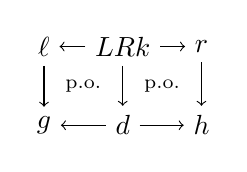
\begin{tikzpicture}
    \node (1t) at (0,1) {$ \ell $};
    \node (2t) at (1,1) {$ LRk $};
    \node (3t) at (2,1) {$ r $};
    \node (1b) at (0,0) {$ g $};
    \node (2b) at (1,0) {$ d $};
    \node (3b) at (2,0) {$ h $};
    \draw [->] (2t) to node [] {\scriptsize{$  $}} (1t);
    \draw [->] (2t) to node [] {\scriptsize{$  $}} (3t);
    \draw [->] (2b) to node [] {\scriptsize{$  $}} (1b);
    \draw [->] (2b) to node [] {\scriptsize{$  $}} (3b);
    \draw [->] (1t) to node [] {\scriptsize{$  $}} (1b);
    \draw [->] (2t) to node [] {\scriptsize{$  $}} (2b);
    \draw [->] (3t) to node [] {\scriptsize{$  $}} (3b);
    \node () at (0.5,0.5) {\scriptsize{p.o.}};
    \node () at (1.5,0.5) {\scriptsize{p.o.}};
  \end{tikzpicture}
  \]
  % 
  the desired square is the horizontal composition of
  %
  \[
    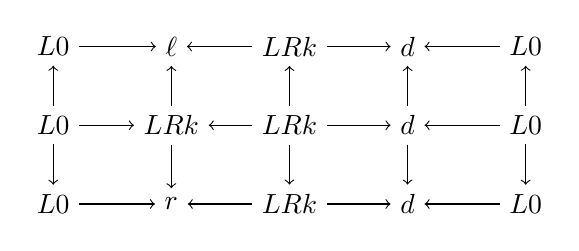
\begin{tikzpicture}
    \begin{scope}
      \node (1t) at (0,2) {$ L0 $};
      \node (2t) at (1.5,2) {$ \ell $};
      \node (3t) at (3,2) {$ LRk $};
      \node (4t) at (4.5,2) {$ d $};
      \node (5t) at (6,2) {$ L0 $};
      \node (1m) at (0,1) {$ L 0 $};
      \node (2m) at (1.5,1) {$ LRk $};
      \node (3m) at (3,1) {$ LRk $};
      \node (4m) at (4.5,1) {$ d $};
      \node (5m) at (6,1) {$ L 0 $};
      \node (1b) at (0,0) {$ L 0 $};
      \node (2b) at (1.5,0) {$ r $};
      \node (3b) at (3,0) {$ LRk $};
      \node (4b) at (4.5,0) {$ d $};
      \node (5b) at (6,0) {$ L 0 $};
      \draw [->] (1t) to node [] {\scriptsize{$  $}} (2t);
      \draw [->] (3t) to node [] {\scriptsize{$  $}} (2t);
      \draw [->] (3t) to node [] {\scriptsize{$  $}} (4t);
      \draw [->] (5t) to node [] {\scriptsize{$  $}} (4t);
      \draw [->] (1m) to node [] {\scriptsize{$  $}} (2m);
      \draw [->] (3m) to node [] {\scriptsize{$  $}} (2m);
      \draw [->] (3m) to node [] {\scriptsize{$  $}} (4m);
      \draw [->] (5m) to node [] {\scriptsize{$  $}} (4m);
      \draw [->] (1b) to node [] {\scriptsize{$  $}} (2b);
      \draw [->] (3b) to node [] {\scriptsize{$  $}} (2b);
      \draw [->] (3b) to node [] {\scriptsize{$  $}} (4b);
      \draw [->] (5b) to node [] {\scriptsize{$  $}} (4b);
      \draw [->] (1m) to node [] {\scriptsize{$  $}} (1t);
      \draw [->] (1m) to node [] {\scriptsize{$  $}} (1b);
      \draw [->] (2m) to node [] {\scriptsize{$  $}} (2t);
      \draw [->] (2m) to node [] {\scriptsize{$  $}} (2b);
      \draw [->] (3m) to node [] {\scriptsize{$  $}} (3t);
      \draw [->] (3m) to node [] {\scriptsize{$  $}} (3b);
      \draw [->] (4m) to node [] {\scriptsize{$  $}} (4t);
      \draw [->] (4m) to node [] {\scriptsize{$  $}} (4b);
      \draw [->] (5m) to node [] {\scriptsize{$  $}} (5t);
      \draw [->] (5m) to node [] {\scriptsize{$  $}} (5b);
    \end{scope}
    \end{tikzpicture}
  \]
  %
  The left square is a generator and the right square is the
  identity on the horizontal arrow $ LRk + L \empty \to d $. The
  square for a derivation $ \dderiv{\deriv{g}{h}}{j} $ is the vertical
  composition of
  %
  \[
    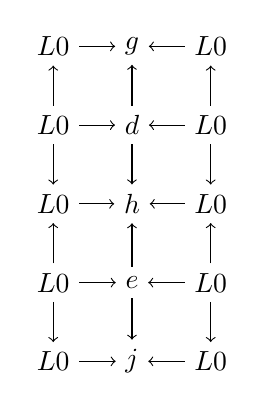
\begin{tikzpicture}
      \node (1t) at (0,4) {$ L 0 $};
      \node (2t) at (1,4) {$ g $};
      \node (3t) at (2,4) {$ L 0 $};
      \node (1m) at (0,3) {$ L 0 $};
      \node (2m) at (1,3) {$ d $};
      \node (3m) at (2,3) {$ L 0 $};
      \node (1b) at (0,2) {$ L 0 $};
      \node (2b) at (1,2) {$ h $};
      \node (3b) at (2,2) {$ L 0 $};
      \node (1bb) at (0,1) {$ L 0 $};
      \node (2bb) at (1,1) {$ e $};
      \node (3bb) at (2,1) {$ L 0 $};
      \node (1bbb) at (0,0) {$ L 0 $};
      \node (2bbb) at (1,0) {$ j $};
      \node (3bbb) at (2,0) {$ L 0 $};
      \draw [->] (1t) to node [] {\scriptsize{$  $}} (2t);
      \draw [->] (3t) to node [] {\scriptsize{$  $}} (2t);
      \draw [->] (1m) to node [] {\scriptsize{$  $}} (2m);
      \draw [->] (3m) to node [] {\scriptsize{$  $}} (2m);
      \draw [->] (1b) to node [] {\scriptsize{$  $}} (2b);
      \draw [->] (3b) to node [] {\scriptsize{$  $}} (2b);
      \draw [->] (1m) to node [] {\scriptsize{$  $}} (1t);
      \draw [->] (1m) to node [] {\scriptsize{$  $}} (1b);
      \draw [->] (2m) to node [] {\scriptsize{$  $}} (2t);
      \draw [->] (2m) to node [] {\scriptsize{$  $}} (2b);
      \draw [->] (3m) to node [] {\scriptsize{$  $}} (3t);
      \draw [->] (3m) to node [] {\scriptsize{$  $}} (3b);
      \draw [->] (1bb) to node [] {\scriptsize{$  $}} (2bb);
      \draw [->] (3bb) to node [] {\scriptsize{$  $}} (2bb);
      \draw [->] (1bbb) to node [] {\scriptsize{$  $}} (2bbb);
      \draw [->] (3bbb) to node [] {\scriptsize{$  $}} (2bbb);
      \draw [->] (1bb) to node [] {\scriptsize{$  $}} (1b);
      \draw [->] (1bb) to node [] {\scriptsize{$  $}} (1bbb);
      \draw [->] (2bb) to node [] {\scriptsize{$  $}} (2b);
      \draw [->] (2bb) to node [] {\scriptsize{$  $}} (2bbb);
      \draw [->] (3bb) to node [] {\scriptsize{$  $}} (3b);
      \draw [->] (3bb) to node [] {\scriptsize{$  $}} (3bbb);
    \end{tikzpicture}
  \]
  %
  The top square is from $ \deriv{g}{h} $ and the second from
  $ \dderiv{h}{j} $.

  Conversely, proceed by structural induction on the generating
  squares of $ \Lang ( \StrCsp_L , P' ) $.  It suffices to show that
  the rewrite relation is preserved by vertical and composition by a
  generating square.  Suppose we have a square
  %
  \[
    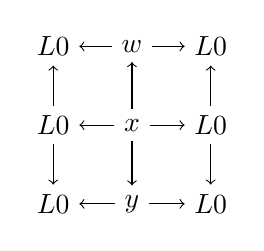
\begin{tikzpicture}
      \node (1t) at (0,2) {$ L 0 $};
      \node (2t) at (1,2) {$ w $};
      \node (3t) at (2,2) {$ L 0 $};
      \node (1m) at (0,1) {$ L 0 $};
      \node (2m) at (1,1) {$ x $};
      \node (3m) at (2,1) {$ L 0 $};
      \node (1b) at (0,0) {$ L 0 $};
      \node (2b) at (1,0) {$ y $};
      \node (3b) at (2,0) {$ L 0 $};
      \draw [->] (2t) to node [] {\scriptsize{$  $}} (1t);
      \draw [->] (2t) to node [] {\scriptsize{$  $}} (3t);
      \draw [->] (2m) to node [] {\scriptsize{$  $}} (1m);
      \draw [->] (2m) to node [] {\scriptsize{$  $}} (3m);
      \draw [->] (2b) to node [] {\scriptsize{$  $}} (1b);
      \draw [->] (2b) to node [] {\scriptsize{$  $}} (3b);
      \draw [->] (1m) to node [] {\scriptsize{$  $}} (1t);
      \draw [->] (2m) to node [] {\scriptsize{$  $}} (2t);
      \draw [->] (3m) to node [] {\scriptsize{$  $}} (3t);
      \draw [->] (1m) to node [] {\scriptsize{$  $}} (1b);
      \draw [->] (2m) to node [] {\scriptsize{$  $}} (2b);
      \draw [->] (3m) to node [] {\scriptsize{$  $}} (3b);
    \end{tikzpicture}
  \]
  % 
  corresponding to a derivation $ \deriv{w}{y} $. Composing this
  vertically with a generating square, which must have form
  %
  \[
    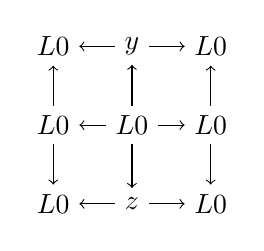
\begin{tikzpicture}
      \node (1t) at (0,2) {$ L 0 $};
      \node (2t) at (1,2) {$ y $};
      \node (3t) at (2,2) {$ L 0 $};
      \node (1m) at (0,1) {$ L 0 $};
      \node (2m) at (1,1) {$ L 0 $};
      \node (3m) at (2,1) {$ L 0 $};
      \node (1b) at (0,0) {$ L 0 $};
      \node (2b) at (1,0) {$ z $};
      \node (3b) at (2,0) {$ L 0 $};
      \draw [->] (2t) to node [] {\scriptsize{$  $}} (1t);
      \draw [->] (2t) to node [] {\scriptsize{$  $}} (3t);
      \draw [->] (2m) to node [] {\scriptsize{$  $}} (1m);
      \draw [->] (2m) to node [] {\scriptsize{$  $}} (3m);
      \draw [->] (2b) to node [] {\scriptsize{$  $}} (1b);
      \draw [->] (2b) to node [] {\scriptsize{$  $}} (3b);
      \draw [->] (1m) to node [] {\scriptsize{$  $}} (1t);
      \draw [->] (2m) to node [] {\scriptsize{$  $}} (2t);
      \draw [->] (3m) to node [] {\scriptsize{$  $}} (3t);
      \draw [->] (1m) to node [] {\scriptsize{$  $}} (1b);
      \draw [->] (2m) to node [] {\scriptsize{$  $}} (2b);
      \draw [->] (3m) to node [] {\scriptsize{$  $}} (3b);
    \end{tikzpicture}
  \]
  %
  corresponding to a production $ 0 \to y + z $ gives
  %
  \[
    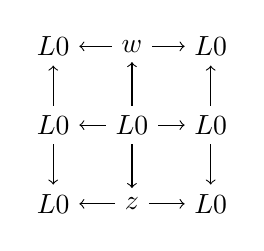
\begin{tikzpicture}
      \node (1t) at (0,2) {$ L 0 $};
      \node (2t) at (1,2) {$ w $};
      \node (3t) at (2,2) {$ L 0 $};
      \node (1m) at (0,1) {$ L 0 $};
      \node (2m) at (1,1) {$ L 0 $};
      \node (3m) at (2,1) {$ L 0 $};
      \node (1b) at (0,0) {$ L 0 $};
      \node (2b) at (1,0) {$ z $};
      \node (3b) at (2,0) {$ L 0 $};
      \draw [->] (2t) to node [] {\scriptsize{$  $}} (1t);
      \draw [->] (2t) to node [] {\scriptsize{$  $}} (3t);
      \draw [->] (2m) to node [] {\scriptsize{$  $}} (1m);
      \draw [->] (2m) to node [] {\scriptsize{$  $}} (3m);
      \draw [->] (2b) to node [] {\scriptsize{$  $}} (1b);
      \draw [->] (2b) to node [] {\scriptsize{$  $}} (3b);
      \draw [->] (1m) to node [] {\scriptsize{$  $}} (1t);
      \draw [->] (2m) to node [] {\scriptsize{$  $}} (2t);
      \draw [->] (3m) to node [] {\scriptsize{$  $}} (3t);
      \draw [->] (1m) to node [] {\scriptsize{$  $}} (1b);
      \draw [->] (2m) to node [] {\scriptsize{$  $}} (2b);
      \draw [->] (3m) to node [] {\scriptsize{$  $}} (3b);
    \end{tikzpicture}
  \]
  %
  which corresponds to a derivation $ \dderiv{\deriv{w}{y}}{z} $.
  Composing horizontally with a generating square
  %
  \[
    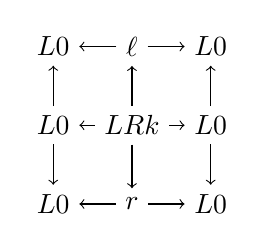
\begin{tikzpicture}
      \node (1t) at (0,2) {$ L 0 $};
      \node (2t) at (1,2) {$ \ell $};
      \node (3t) at (2,2) {$ L 0 $};
      \node (1m) at (0,1) {$ L 0 $};
      \node (2m) at (1,1) {$ LRk $};
      \node (3m) at (2,1) {$ L 0 $};
      \node (1b) at (0,0) {$ L 0 $};
      \node (2b) at (1,0) {$ r $};
      \node (3b) at (2,0) {$ L 0 $};
      \draw [->] (2t) to node [] {\scriptsize{$  $}} (1t);
      \draw [->] (2t) to node [] {\scriptsize{$  $}} (3t);
      \draw [->] (2m) to node [] {\scriptsize{$  $}} (1m);
      \draw [->] (2m) to node [] {\scriptsize{$  $}} (3m);
      \draw [->] (2b) to node [] {\scriptsize{$  $}} (1b);
      \draw [->] (2b) to node [] {\scriptsize{$  $}} (3b);
      \draw [->] (1m) to node [] {\scriptsize{$  $}} (1t);
      \draw [->] (2m) to node [] {\scriptsize{$  $}} (2t);
      \draw [->] (3m) to node [] {\scriptsize{$  $}} (3t);
      \draw [->] (1m) to node [] {\scriptsize{$  $}} (1b);
      \draw [->] (2m) to node [] {\scriptsize{$  $}} (2b);
      \draw [->] (3m) to node [] {\scriptsize{$  $}} (3b);
    \end{tikzpicture}
  \]
  %
  corresponding with a production $ LRk \to \ell + r $ results in the
  square
  %
  \[
    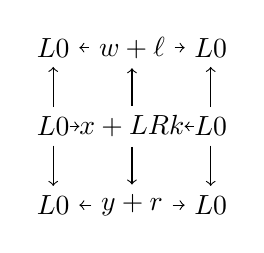
\begin{tikzpicture}
      \node (1t) at (0,2) {$ L 0 $};
      \node (2t) at (1,2) {$ w + \ell $};
      \node (3t) at (2,2) {$ L 0 $};
      \node (1m) at (0,1) {$ L 0 $};
      \node (2m) at (1,1) {$ x + LRk $};
      \node (3m) at (2,1) {$ L 0 $};
      \node (1b) at (0,0) {$ L 0 $};
      \node (2b) at (1,0) {$ y + r $};
      \node (3b) at (2,0) {$ L 0 $};
      \draw [->] (2t) to node [] {\scriptsize{$  $}} (1t);
      \draw [->] (2t) to node [] {\scriptsize{$  $}} (3t);
      \draw [->] (2m) to node [] {\scriptsize{$  $}} (1m);
      \draw [->] (2m) to node [] {\scriptsize{$  $}} (3m);
      \draw [->] (2b) to node [] {\scriptsize{$  $}} (1b);
      \draw [->] (2b) to node [] {\scriptsize{$  $}} (3b);
      \draw [->] (1m) to node [] {\scriptsize{$  $}} (1t);
      \draw [->] (2m) to node [] {\scriptsize{$  $}} (2t);
      \draw [->] (3m) to node [] {\scriptsize{$  $}} (3t);
      \draw [->] (1m) to node [] {\scriptsize{$  $}} (1b);
      \draw [->] (2m) to node [] {\scriptsize{$  $}} (2b);
      \draw [->] (3m) to node [] {\scriptsize{$  $}} (3b);
    \end{tikzpicture}
  \]
  %
  But $ \deriv{w+\ell}{y+r} $ as seen in Lemma
  \ref{thm:rewrite-rel-is-additive}. 

\end{proof}


% ~~~~~~~~~~~~~~~~~~~~~~~~~~~~~~~~~~~~~~~~
% 
% ~~~~~~~~~~~ bibliography ~~~~~~~~~~~~~~~
% 
% ~~~~~~~~~~~~~~~~~~~~~~~~~~~~~~~~~~~~~~~~

\begin{thebibliography}{99}
  % use APA style
  % \bibitem{1st-citation}

\bibitem{StrCsp} J.~Baez, K.~Courser. Structured cospans. \emph{In preparation}.

\bibitem{NetMods} J.~Baez, J.~Foley, J.~Moeller, B.~Pollard. Network
  Models. \emph{arXiv preprint} arXiv:1711.00037. 2017.
  
\bibitem{PassiveNets} J.~Baez, B.~Fong. A compositional framework for passive linear networks. \emph{arXiv preprint} arXiv:1504.05625. 2015.

\bibitem{MrkvProc} J.~Baez, B.~Fong, B.~Pollard. A compositional
  framework for Markov processes. \emph{J.~Math.~Phys.} 57, No.~3:
  033301. 2016.
  
\bibitem{RxNets} J.~Baez, B.~Pollard. A compositional framework for
  reaction networks. \emph{Rev. Math. Phys.} 29, No.~9, 1750028. 2017.

\bibitem{OpenPetri} J.~Baez, J.~Master. Open Petri Nets. \emph{arXiv preprint} arXiv:1808.05415. 2018.
  
\bibitem{Chomsky} N.~Chomsky. On Certain Formal Properties of Grammars.
\emph{Inf.~Control}. No.~2. 137-167. 1959. 
  
\bibitem{Cic_SpCsp} D.\ Cicala. Spans of cospans. \emph{Theory Appl.\
    Categ.} 33, No.\ 6, 131--147. 2018.

\bibitem{CicCour_SpCspTopos} D.\ Cicala and K.\ Courser. Spans of
  cospans in a topos. \emph{Theory Appl.\ Categ.} 33, No.\ 1,
  1--22. 2018.

\bibitem{DixKiss_OpenGraphs} L.\ Dixon, and A.\ Kissinger. Open-graphs
  and monoidal theories. \emph{Math.\ Structures Comput.\ Sci.},
  \textbf{23}, No.\ 2, 308--359. 2013.

\bibitem{Ehrig_GraphGram} H.\ Ehrig, M.\ Pfender, and H.J.\
  Schneider. Graph-grammars: An algebraic approach. In \emph{Switching
    and Automata Theory, 1973. SWAT'08. IEEE Conference Record of 14th
    Annual Symposium on}, 167--180. IEEE. 1973.
  
\bibitem{DecorCsp} B.\ Fong. Decorated cospans. \emph{Theory
    Appl.\ Categ.} 30, Paper No.\ 33, 1096--1120. 2015.
          
\bibitem{Gadd_IndGraphTrans} F.\ Gadducci, R.\ Heckel. An inductive
  view of graph transformation.\emph{International Workshop on
    Algebraic Development Techniques}. 223--237. Springer, Berlin. 1998.

\bibitem{DblPushoutRevis} A.~Habel, J.~M\:{u}ller,
  D.~Plump. Double-pushout graph transformation
  revisited. \emph{Math. Structures Comput. Sci.}
  11. No.~5. 637--688. 2001).
  
\bibitem{LackSobo_Adhesive} S.\ Lack, and P.\ Soboci\'{n}ski. Adhesive
  categories. In \emph{International Conference on Foundations of
    Software Science and Computation Structures}, 273--288. Springer,
  Berlin, Heidelberg. 2004.

\bibitem{LackSobo_ToposIsAdh} S.~Lack, P.~Soboci\'{n}ski. Toposes are adhesive. \emph{International Conference on Graph Transformation}. Springer, Berlin, Heidelberg. 2006.

\bibitem{ShulDblCat} M.~Shulman. Constructing symmetric monoidal bicategories. \emph{arXiv preprint} arXiv:1004.0993. 2010.
  
\bibitem{Wraith_ArtinGlue} G.\ Wraith. Artin gluing. \emph{J.\ Pure
    Appl.\ Algebra} \textbf{4}, 345--348. 1974.

\end{thebibliography}

\end{document}
